\documentclass[a4paper,10pt]{report}

\usepackage[utf8]{inputenc}
\usepackage[italian]{babel}
\usepackage{amsmath}
\usepackage{amsfonts}
\usepackage{xfrac}
\usepackage{bm}
\usepackage{hyperref}

\usepackage{amsmath}
\usepackage{array}
\usepackage{amstext}
\usepackage{amsthm}
\usepackage{enumitem}
\usepackage{fancyhdr}
\usepackage{eurosym}
\usepackage{amsmath,amssymb}
\usepackage{graphicx}
\usepackage{listings}
\usepackage{lstautogobble}
\usepackage{changepage}
\usepackage{multicol}
\usepackage{adjustbox}
\usepackage{caption}
\usepackage[labelformat=simple]{subcaption}
\renewcommand\thesubfigure{(\alph{subfigure})}
%\usepackage{easytable}
%\usepackage{color}

%%editing
\usepackage{todonotes}

\lstdefinestyle{customc}{
  belowcaptionskip=1\baselineskip,
  breaklines=true,
  %frame=L,
  xleftmargin=\parindent,
  language=C++,
  showstringspaces=false,
  basicstyle=\footnotesize\ttfamily,
  keywordstyle=\bfseries\color{green!40!black},
  commentstyle=\itshape\color{red},
  identifierstyle=\color{blue},
  stringstyle=\color{orange},
}

\lstset{style=customc}


\hypersetup{
    colorlinks=false,
    pdfborder={0 0 0},
}

\usepackage{listings}
\usepackage{lstautogobble}

\lstset{basicstyle=\ttfamily,
  mathescape=true,
  escapeinside=||,
  autogobble}
  
\setlength{\parindent}{0pt}

\newcommand{\der}[2]{\frac{\partial #1}{\partial #2}}
\newcommand{\dder}[2]{\frac{\partial^2 #1}{\partial #2^2}}
\newcommand{\dmix}[3]{\frac{\partial^2 #1}{\partial #2 \partial #3}}

\theoremstyle{plain}
\newtheorem{theorem}{Teorema}[chapter]
\newtheorem{prop}{Proposizione}[chapter]
\newtheorem{lem}{Lemma}[chapter]
\newtheorem{corollario}{Corollario}[section]

\theoremstyle{definition}
\newtheorem{definition}{Definizione}[chapter]
\newtheorem{notazione}{Notazione}[chapter]

\theoremstyle{remark}
\newtheorem{osservazione}{Osservazione}[chapter]
\newtheorem{esempio}{Esempio}%[chapter]

\DeclareMathOperator{\Div}{Div}

\begin{document}

\thispagestyle{empty}

	\begin{center}
	 {\large{\textbf{POLITECNICO DI MILANO}\\
             Corso di Laurea Magistrale di Ingegneria Matematica\\
             Facolt\`a di Ingegneria dei Sistemi\\
             }}
	\end{center}

	\vspace{1cm}
	\begin{figure}[htbp]
	\begin{center}
	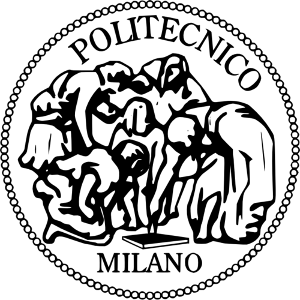
\includegraphics[width=4cm]{img/poli_logo.png}
	\end{center}
	\end{figure}
	
	\vspace{1cm}
	\begin{center}
	{\LARGE{Progetto di Programmazione Avanzata per il Calcolo Scientifico:}}
	\end{center}
	%\color{white}
	\vspace{2cm}
	\begin{center}
	{\LARGE{\textbf{Metodo a elementi finiti per il pricing di opzioni multi-asset con modelli di L\'evy}}}
	\end{center}
	
	%\color{black}
	%\vspace{2.5 cm}
	\begin{table}[hb!]
	\begin{center}
	\begin{tabular}{p{8cm}p{7cm}}
	& \\
  	& \\
  	& {\large Nahuel Foresta, matr. 798775}\\
	& {\large Giorgio G. Re, matr. 799260}\\
	\end{tabular}
	\end{center}
	\end{table}
	\begin{center}
	\vspace{3cm}
	\large{Anno Accademico 2012-2013}
	\end{center}

	\clearpage
	\thispagestyle{empty}
	
	\clearpage

\clearpage
\thispagestyle{plain}
\par\vspace*{.35\textheight}{\raggedleft An approximate answer to the right problem is worth a good deal more than an exact answer to an approximate problem.\par}
\par\vspace{1cm}{\raggedleft John Tukey\par}

\tableofcontents
\listoffigures
\listoftables

\chapter*{Introduzione}

Lo scopo di questo progetto è creare un piccolo \emph{tool} scritto in c++ che possa risolvere il problema di \emph{pricing} per alcuni derivati finanziari, tramite la soluzione di equazioni integro-differenziali. Abbiamo quindi sviluppato la base di una libreria (molto semplice ma completamente funzionale) per il calcolo del prezzo di opzioni usando il metodo degli elementi finiti. Il tutto è basato sulla libreria ad elementi finiti esterna \textsf{deal.ii}, che fornisce pi\`u del necessario per la base di un programma che sfrutti il metodo degli elementi finiti sui quadrilateri. Cos\`i come la libreria \textsf{deal.ii}, il progetto \`e una libreria \emph{template}, nel senso che quasi tutti gli oggetti utilizzati sono \emph{templatizzati} sulla dimensione. Combinando l'uso di \textsf{deal.ii} per trattare la parte differenziale, e le nostre aggiunte per trattare la parte integrale, abbiamo creato una libreria che permette di calcolare il prezzo degli oggetti base (opzioni \emph{call} e \emph{put}) in una e due dimensioni, ma che al tempo stesso fornisce il macchinario per risolvere altri problemi simili con l'aggiunta di pochissimo codice, attraverso meccanismi di ereditarietà. Oltre al problema classico (in gergo finanziario chiamato opzione europea), abbiamo anche aggiunto la risoluzione di un problema di tipo opzione americana, in cui la soluzione deve stare sopra un dato limite, ossia un problema con ostacolo.\\

Una delle motivazioni che ci ha spinti a intraprendere questo progetto è la totale assenza di codici che risolvano questi problemi ad elementi finiti in più di una dimensione. Questo si spiega con il fatto che, essendo i domini quasi sempre dei rettangoli, i metodi basati sulle differenze finite, comunque pi\`u semplici da trattare, sono molto più diffusi. Da un punto di vista di prestazioni, le differenze finite non presentano particolari vantaggi sugli elementi finiti. Gli elementi finiti invece, seppur più difficili da usare, possono in alcuni casi essere più convenienti e pi\`u precisi, sopratutto per i problemi in più dimensioni. Un esempio è l'adattività locale di griglia, come vedremo in seguito.\\

Nei Capitolo 1 e 2 introdurremo da un punto di vista finanziario il problema, ricavando le equazioni di nostro interesse ed esplicitando le condizioni al bordo e la condizione finale. Nel Capitolo 3 invece descriveremo da un punto di vista numerico gli algoritmi e le discretizzazioni usate per risolvere i nostri problemi differenziali nei due cambi di variabile che abbiamo sfruttato. Il Capitolo 4 descrive poi gli strumenti utilizzati per la stesura del codice, quali \textsf{deal.ii}, \textsf{CMake}, GitHub. Nel capitolo 5 esporremo la struttura del nostro codice e in particolare parleremo delle classi principali che abbiamo scritto, oltre a fornire una piccola guida per un primo utilizzo della nostra libreria. Nel Capitolo 6 poi analizzeremo tramite alcuni programmi test i risultati ottenuti dai nostri codici. Nel Capitolo 7 parleremo di possibili estensioni al nostro codice, con due esempi. Infine nel Capitolo 8 giungeremo a delle conclusioni sul lavoro fatto e in particolare sull'utilizzo del metodo a elementi finiti rispetto alle differenze finite.

\chapter{Modello di Black \& Scholes}

\section{Introduzione}
In questo capitolo descriviamo i modelli basilari utilizzati per descrivere il mercato finanziario, seguendo le argomentazioni di Merton (1973), trattate in \cite{bjork2009arbitrage}. Consideriamo quindi un mercato finanziario molto semplificato, costituito da un titolo \emph{risk-free} descritto dal processo $B$ e un titolo azionario con valore pari al processo $S$. Definiamo quindi questi due processi.
\begin{definition}
Sia $(\Omega,\mathcal{F},\mu)$ uno spazio misurabile e sia $\mathcal{F}_{t\in [ 0,T ]}$ una filtrazione. Allora, il processo B descrive il valore di un titolo \emph{risk-free} se la sua dinamica \`e del tipo: $$dB(t)=r(t)B(t)dt,$$dove $r$ \`e un qualsiasi processo $\mathcal{F}_t$-adattato.
\end{definition}
La caratteristica pi\`u importante quindi dei processi \emph{risk-free} \`e l'assenza di aleatoriet\`a data da un processo stocastico casuale. Integrando l'equazione precedente, otteniamo: $$B(t)=B(0)\int_0^tr(s)ds.$$ Un caso particolare \`e quello in cui $r$ \`e una costante deterministica, in tal modo $B$ descrive l'andamento di un'obbligazione.\\\\Assumiamo poi che la dinamica di $S$ sia data da: $$dS(t)=S(t)\mu(t,S(t))dt+S(t)\sigma(t,S(t))dW(t),$$ in cui $W_t$ \`e un processo di Wiener (cio\`e un moto browniano) e $\mu$ e $\sigma$ due funzioni deterministiche. La funzione $\sigma$ \`e detta volatilit\`a del titolo, $\mu$ \`e il tasso di ritorno di $S$.
%\begin{osservazione}
%Osserviamo la differenza fra il tasso di ritorno di un titolo \emph{risk-free} e quello di un titolo rischioso. Il tasso di $B$ \`e: $$\frac{dB(t)}{B(t)dt}=r(t),$$ ovvero totalmente deterministico, mentre quello di $S$ \`e dato da: $$\frac{dS(t)}{S(t)dt}=\mu(t,S(t))+\sigma(t,S(t)) \frac{dW(t)}{dt},$$ oggetto che non \`e osservabile al tempo $t$. Esso \`e infatti costituito da $\mu$ e $\sigma$ che sono entrambi osservabili al tempo $t$, pi\`u un rumore bianco $W(t)$ che \`e del tutto casuale. Quindi, al contrario del titolo \emph{risk-free}, l'azione ha un tasso di ritorno stocastico, anche su una scala infinitesima.
%\end{osservazione}
Passiamo ora a definire il modello di \emph{Black\&Scholes}.
\begin{definition}
Il modello di \emph{Black\&Scholes} consiste di due titoli con le seguenti dinamiche:
\begin{align*}
dB(t)&=rB(t)dt,\\
dS(t)&=\mu S(t)dt+\sigma S(t)dW(t),
\end{align*}
dove $r$, $\mu$ e $\sigma$ sono costanti deterministiche.
\end{definition}

\section{Strumenti derivati e Opzioni}
In questa sezione definiamo gli strumenti derivati e, in particolare, le opzioni che abbiamo trattato nel progetto.
\begin{definition}
In finanza, \`e denominato strumento derivato ogni contratto o titolo il cui valore si basa sul valore di mercato di un altro titolo o strumento finanziario, detto sottostante (ad esempio, azioni, valute, tassi di interesse o derivati stessi).
\end{definition}
Definiamo ora il titolo derivato pi\`u semplice, ovvero l'opzione \emph{call} europea.
\begin{definition}
Un'opzione \emph{call} europea con prezzo di esercizio (o \emph{strike price}) $K$ e scadenza $T$ sul sottostante $S$ \`e un contratto finanziario derivato con le seguenti caratteristiche:
\begin{itemize}
\item il titolare del contratto ha, al tempo $T$, il diritto di acquistare un'azione del sottostante al prezzo $K$ dal sottoscrittore del contratto, qualsiasi sia il valore del sottostante $S$ al tempo $T$;
\item il titolare del contratto non ha alcun obbligo di acquistare un'azione del sottostante al tempo $T$;
\item il diritto di acquistare un'azione del sottostante pu\`o essere esercitato solo al tempo $T$.
\end{itemize}
\end{definition}
Osserviamo che la scadenza del contratto e il prezzo d'esercizio sono stabiliti alla stipula del contratto, che per noi sar\`a tipicamente $t=0$.\\Oltre alle opzioni \emph{call} europee, esistono opzioni \emph{put} europee, le quali danno al titolare del contratto il diritto a vendere (anzich\'e comprare) un dato titolo azionario a un prezzo fissato $K$. Le opzioni americane invece (\emph{call} o \emph{put} che siano), permettono di esercitare il diritto all'acquisto o alla vendita dell'azione in ogni istante di tempo $t\in[0,T]$.
\begin{esempio}
Supponiamo di possedere un'opzione \emph{call} con scadenza $T=1$ anno, \emph{strike price} $K=100$\officialeuro$ $ e un sottostante che al tempo $t=0$ vale $S_0=100$\officialeuro. Allora, se fra un anno $S_T=120$\officialeuro$ $, eserciteremo l'opzione, acquistando il sottostante per un prezzo pari a $K=100$\officialeuro$ $, e il sottoscrittore del contratto pagher\`a i rimenenti $S_T-K=20$\officialeuro$ $. Se invece $S_T=80$\officialeuro$ $ non eserciteremo l'opzione, ottenendo un guadagno pari a 0.
\end{esempio}
Osserviamo quindi che il valore a scadenza, cio\`e il \emph{payoff}, dell'opzione dipende soltanto dal valore del sottostante. Definiamo quindi il
\emph{payoff} come variabile aleatoria in funzione di $S$.
\begin{definition}
Sia $S$ il processo stocastico che descrive l'andamento di un titolo azionario, allora il \emph{payoff} di un'opzione scritta su $S$ con scadenza $T$ e \emph{strike} $K$ \`e una variabile aleatoria $\mathcal{X}\in\mathcal{F}_T$, e: $$\mathcal{X}=\Phi(S_T).$$
\end{definition}
Per esempio, il \emph{payoff} delle opzioni \emph{call} e \emph{put} europee \`e:
\begin{align*}
\Phi_C(S_T)&=\max(S_T-K,0),\\
\Phi_P(S_T)&=\max(K-S_T,0).
\end{align*}
La domanda che ci poniamo ora \`e la seguente: qual \`e il prezzo equo di un'opzione? Ovvero, quanto occorre pagare oggi per avere il diritto ma non l'obbligo di acquistare al tempo $T$ un'azione a un prezzo fissato $K$?

\section{L'equazione di \emph{Black\&Scholes}}
Vi sono molti modi per ricavare l'equazione di \emph{Black\&Scholes}: presentiamo qui il modo pi\`u semplice e veloce.\\\\Prima di ricavare l'equazione spendiamo qualche riga per descrivere il concetto di neutralit\`a al rischio in finanza. Un operatore economico si dice neutrale al rischio quando le sue preferenze lo rendono indifferente al compiere un'azione il cui risultato \`e una quantit\`a aleatoria, oppure compiere un'azione il cui risultato \`e il valore atteso della quantit\`a aleatoria stessa.\\Per esempio, per un soggetto neutrale al rischio sono indifferenti le seguenti situazioni:
\begin{itemize}
\item avere $1$\officialeuro$ $ con probabilit\`a 1;
\item giocare a una lotteria in cui il soggetto pu\`o ricevere $2$\officialeuro$ $ con probabilit\`a $\sfrac{1}{2}$ o $0$\officialeuro$ $ con probabilit\`a $\sfrac{1}{2}$.
\end{itemize}
Nel primo caso infatti, egli ottiene sempre $1$\officialeuro$ $, nel secondo ottiene in media $1$\officialeuro$ $. Perci\`o per un soggetto neutrale al rischio queste situazioni sono indifferenti.\\Quando ci occupiamo di \emph{pricing} di derivati, ci poniamo sempre nell'ipotesi di neutralit\`a al rischio. In particolare,
\begin{enumerate}
\item assumiamo che il termine di deriva $\mu$ del modello $S$ sia pari al tasso di interesse \emph{risk-free} $r$, cio\`e poniamo: $$dS(t)=rS(t)dt+\sigma S(t)dW(t);$$
\item calcoliamo il valore atteso del \emph{payoff}, cio\`e $\mathbb{E}\left[\Phi(S_T)|\mathcal{F}_t\right]$;
\item scontiamo il valore atteso del \emph{payoff} con il tasso di interesse $r$.
\end{enumerate}
Sia quindi $C:\mathbb{R}^+\times[0,T]\rightarrow\mathbb{R}^+$, $C=C(S(t),t)$ il processo stocastico che descrive il valore di un'opzione. In particolare, se consideriamo una \emph{call} europea,
$$C(S,t)=e^{(-r(T-t))}\mathbb{E}\left[\max(S_T-K,0)|\mathcal{F}_t\right].$$
Data la dinamica di $S$, se applichiamo a questa quantit\`a il Lemma di It$\hat{o}$, otteniamo la seguente equazione: $$dC(S,t)=\left(\der{C}{t}+r S \der{C}{S} +\frac{1}{2}S^2\dder{C}{S}\right)dt+\sigma S \der{C}{S}dW(t).$$
Dall'altro lato per\`o, per la \emph{risk-neutrality}, la deriva di $C$, come quella di ogni titolo finanziario, dovr\`a essere pari a $rC$, quindi:$$\der{C}{t}+r S \der{C}{S} +\frac{1}{2}S^2\dder{C}{S}=rC.$$
Riassumendo, posti $C=C(S,t)$ e $P=P(S,t)$ i processi che descrivono il prezzo di opzioni \emph{call} e \emph{put}, otteniamo le seguenti equazioni alle derivate parziali con le rispettive condizioni finali e condizioni al bordo:
\begin{equation}
\begin{cases}
\displaystyle
\der{C}{t}+r S \der{C}{S} +\frac{1}{2}S^2\dder{C}{S}=rC,\\
C(S,T)=\max(S_T-K,0),\\
C(0,t)=0,\qquad\quad\qquad\forall t\in[0,T],\\
\lim\limits_{S\to\infty}C(S,t)=\infty,\qquad\forall t\in[0,T],
\end{cases}
\label{callbs1d}
\end{equation}
e
\begin{equation}
\begin{cases}
\displaystyle
\der{P}{t}+r S \der{P}{S} +\frac{1}{2}P^2\dder{P}{S}=rP,\\
P(S,T)=\max(K-S_T,0),\\
P(0,t)=K,\qquad\qquad\forall t\in[0,T]\\
\lim\limits_{S\to\infty}P(S,t)=0,\qquad\forall t\in[0,T].
\end{cases}
\label{putbs1d}
\end{equation}
Come possiamo osservare, si tratta di equazioni paraboliche \emph{backward} con dato finale. Il prezzo dell'opzione sar\`a dato dalla soluzione C o P, valutate in $S_t=S_0$, ovvero il valore dell'azione oggi, e in $t=0$.

\section{Opzioni Basket}
Un altro tipo di opzioni scambiate sui mercati finanziari sono le opzioni basket, il cui \emph{payoff} dipende cio\`e da due o pi\`u sottostanti. In particolare, in questo progetto ci siamo concentrati sul \emph{pricing} di opzioni basket 2D, con i seguenti valori finali: $$C(S_1, S_2, T)=\max(S_{1,T}+S_{2,T}-K,0)$$ per la \emph{call} e: $$P(S_1, S_2, T)=\max(K-S_{1,T}-S_{2,T},0)$$ per la \emph{put}, dove $S_{1,T}$ e $S_{2,T}$ sono i valori al tempo $T$ dei due sottostanti $S_1$ e $S_2$.\\L'equazione che si ottiene con procedimenti analoghi a quelli mostrati nella sezione precedente \`e la seguente:
\begin{equation}
\der{C}{t}+rS_1\der{C}{S_1}+rS_2\der{C}{S_2}+\frac{\sigma^2_1}{2}S_1^2\dder{C}{S_1}+\frac{\sigma^2_2}{2}S_2^2\dder{C}{S_2}+\rho\sigma_1\sigma_2\dmix{C}{S_1}{S_2}=rC,
\label{pde2d}
\end{equation}
in cui $C:\mathbb{R}^+\times\mathbb{R}^+\times[0,T]\rightarrow\mathbb{R}^+$, $C=C(S_1(t), S_2(t),t)$, $\sigma_1$ e $\sigma_2$ sono le volatilit\`a dei due sottostanti e $\rho$ \`e il coefficiente di correlazione fra $S_1$ e $S_2$.

\section{Opzioni Americane: il problema con frontiera libera}
Le opzioni americane differiscono dalle europee poich\'e consentono di esercitare l'opzione non solo in $T$, bens\`i in qualsiasi istante di tempo dalla stipula del contratto alla sua scadenza. Quindi, proprio perch\'e danno al titolare del contratto dei diritti aggiuntivi, \`e facile capire che vale la seguente relazione: $$V^{Am}\geq V^{Eu},$$ ovvero il valore di un'opzione americana \`e sempre superiore al valore dell'europea corrispondente. In particolare, il valore dell'opzione americana \`e sempre pari o superiore al valore del \emph{payoff}. L'opzione europea, infatti, pu\`o avere un valore inferiore al \emph{payoff}, ma questo non pu\`o succedere per le americane. Infatti, se cos\`i non fosse, potremmo acquistare un'azione e una \emph{put} su questa azione ed esercitare immediatamente, ottenendo un guadagno certo senza correre alcun rischio. Per questo valgono i seguenti vincoli:
\begin{align}
C^{Am}(S,t)&\geq \max(S_T-K,0)\qquad\forall t\in[0,T],\\
P^{Am}(S,t)&\geq \max(K-S_T,0)\qquad\forall t\in[0,T].
\label{putbound}
\end{align}
\begin{figure}[h!]
\begin{center}
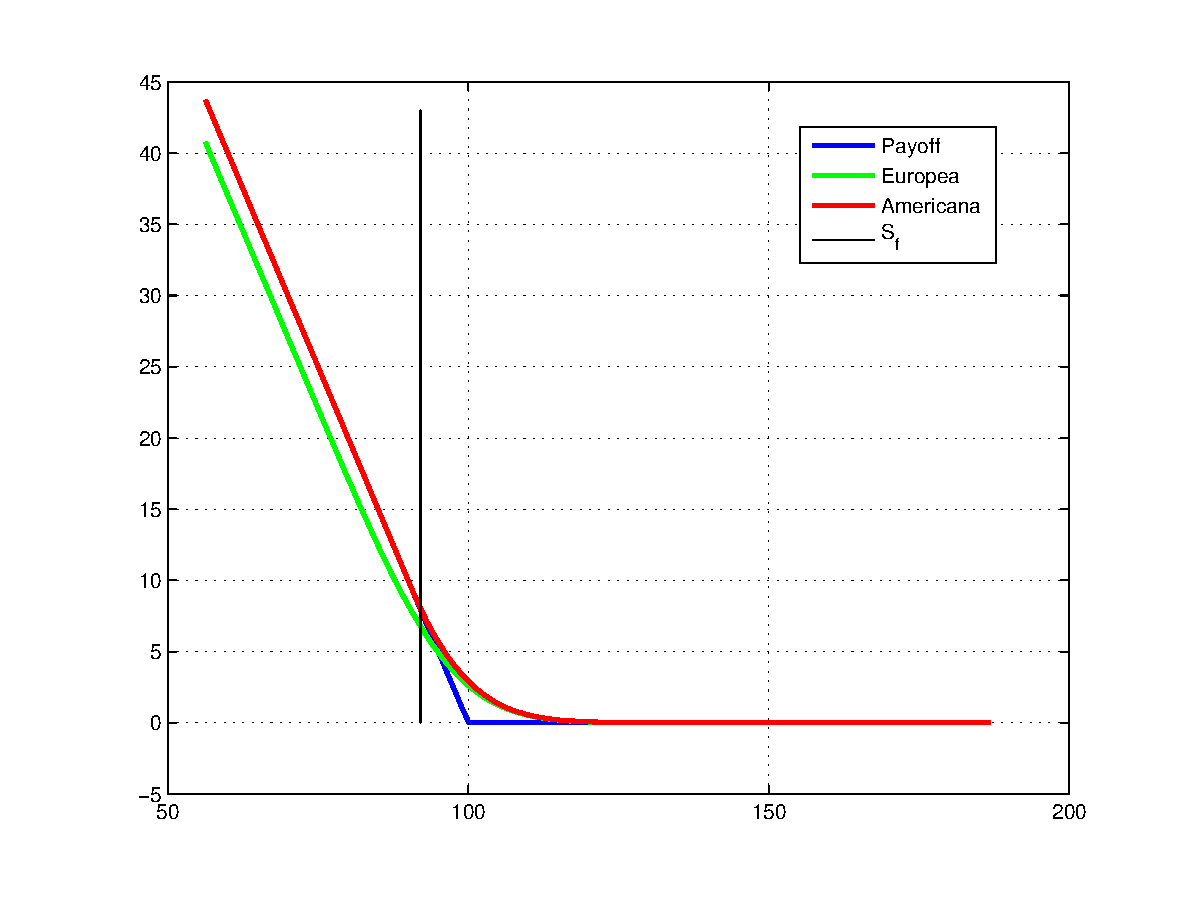
\includegraphics[width=12cm]{img/putam.eps}
\caption{Opzioni Americane vs. Opzione Europee}
\label{putamfig}
\end{center}
\end{figure}
Consideriamo ora il comportamento della \emph{put} nella parte sinistra del grafico riportato in figura \ref{putamfig}. Senza la possibilt\`a di esercizio anticipato, $P^{Eu}<K-S$, ma per la disuguaglianza \ref{putbound}, $P^{Am}=K-S$. Nella parte destra della curva, invece, vale $P^{Am}\geq \max(K-S,0)$. Quindi, per la continuit\`a e la monotonia di $P^{Am}$, la curva dovr\`a toccare il \emph{payoff} in un punto $S_f(t)$, $0<S_f(t)<K$. Questo punto \`e definito da:
\begin{align*}
P^{Am}(S,t)&>\max(K-S,0)\qquad S>S_f(t),\\
P^{Am}(S,t)&=K-S\qquad\qquad\quad S<S_f(t).
\end{align*}
Quindi, $\forall t\in[0,T]$, dobbiamo determinare il punto $S_f(t)$, attraverso il quale passa la retta che separa l'area in cui $P^{Am}=$\emph{payoff} da qualla in cui $P^{Am}>$\emph{payoff}. Poich\'e a priori questa frontiera \`e ignota, questo problema \`e detto ``a frontiera libera''.\\\\Per le \emph{call} americane la situazione \`e differente, poich\'e $C^{Eu}\geq \max(S_T-K,0)$\footnote{Questa relazione si calcola immediatamente sfruttando alcune semplici relazioni che legano $C$, $S$ e $K$. In particolare, nel qual caso: $C^{Am}\geq C^{Eu} \geq S-Ke^{-r(T-t)} > S-K$}. Perci\`o il prezzo di una \emph{call} americana \`e identico a quello di un'europea e in questo caso non si pone il problema con frontiera libera.\\\\Formalmente, l'equazione differenziale che occorre risolvere per trovare il prezzo di una \emph{put} americana \`e la seguente:
\begin{equation}
\begin{cases}
\displaystyle
\der{P}{t}+r S \der{P}{S} +\frac{1}{2}S^2\dder{P}{S}\leq rP,\\
P(S,t)\geq \max(K-S_T,0),\\
P(S,T)=\max(K-S_T,0),\\
P(0,t)=K,\qquad\qquad\forall t\in[0,T]\\
\lim\limits_{S\to\infty}P(S,t)=0,\qquad\forall t\in[0,T].
\end{cases}
\label{putam1d}
\end{equation}
%nel caso monodimensionale, occorre aggiungere ai problemi \ref{callbs1d} e \ref{putbs1d} rispettivamente i seguenti vincoli: $$C(S,t)\geq \max(S_t-K,0), \qquad\forall t\in[0,T],$$ e $$P(S,t)\geq \max(K-S_t,0),\qquad\forall t\in[0,T].$$

\section{Difetti del modello di \emph{Black\&Scholes}}
Il modello di \emph{Black\&Scholes}, nonostante sia molto utilizzato in finanza, presenta alcuni problemi e pu\`o essere pericoloso utilizzarlo per valutare strumenti derivati. In particolare, empiricamente, si evidenziano le seguenti problematiche:
\begin{itemize}
\item il valore di $S$ pu\`o essere discontinuo, ovvero \`e possibile che il sottostante presenti dei "salti";
\item le code della distribuzione dei log-rendimenti dovrebbero essere normali, ma non lo sono: i valori delle code sono infatti pi\`u probabili di quanto ipotizzato dal modello, inoltre le code non sono simmetriche poich\'e presentano un'asimmetria verso i rendimenti negativi;
\item i log-rendimenti inoltre non hanno distribuzioni indipendenti: nelle serie storiche si osservano infatti i cosiddetti \emph{cluster}, ovvero periodi in cui la volatilit\`a \`e alta e rimane alta alternati a periodi con una volatilit\`a che rimane ridotta per lungo tempo;
\item in figura \ref{smile} \`e rappresentato il grafico volatilit\`a vs. \emph{moneyness}\footnote{La \emph{moneyness} di un'opzione \`e il rapporto fra prezzo del sottostante in $t=0$ e \emph{Strike}, ovvero $\sfrac{S_0}{K}$.}. In esso possiamo osservare che il valore della volatilit\`a non rimane costante al variare dei prezzi di esercizio, bens\`i presenta una forma convessa. Questo fenomeno \`e noto come \emph{smile} di volatilit\`a.
\end{itemize}
\begin{figure}[htbp!]
\begin{center}
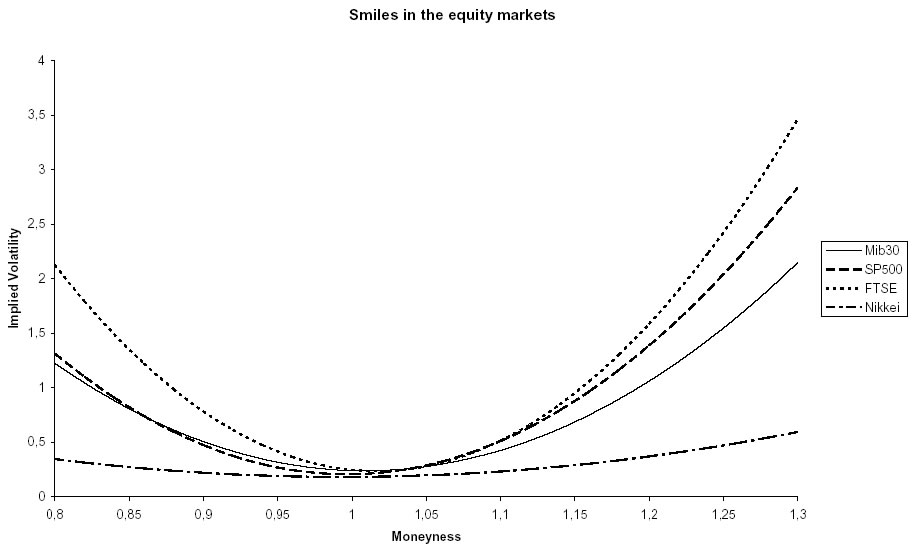
\includegraphics[width=11cm]{img/smile.jpg}
\caption{\emph{Smile} di volatilit\`a}
\label{smile}
\end{center}
\end{figure}
Nel prossimo capitolo introdurremo una classe pi\`u ampia di processi stocastici, cio\`e i processi di L\'evy, e descriveremo dei modelli che permettono di risolvere alcuni dei problemi sopra descritti. Questi modelli danno luogo a equazioni simili a quella di \emph{Black\&Scholes} (PDE) con l'aggiunta per\`o di un termine integrale, per questo le chiameremo Equazioni Integro-Differenziali alle Derivate Parziali (PIDE).

\chapter{Processi di L\'evy e Modelli di Kou e Merton}
\section{Introduzione}
In questo secondo capitolo introduciamo i processi di L\'evy, una classe pi\`u ampia di processi stocastici che permettono di descrivere con pi\`u accuratezza il comportamento di un titolo azionario. Elenchiamo ora alcune definizioni e un teorema che ci permettono di definire i nuovi modelli.
\begin{definition}
Sia $(\Omega, \mathcal{F}, \mu)$ uno spazio misurabile e sia $\mathcal{F}_{t\in[0,T]}$ una filtrazione. Sia $X_t$ un processo stocastico \emph{cadlag}\footnote{Ricordiamo che un processo \`e detto \emph{cadlag} se ha traiettorie continue a destra e limitate a sinistra.}, allora $X_t$ \`e di L\'evy se:
\begin{enumerate}
\item $X_0=0$,
\item ha incrementi indipendenti,
\item ha incrementi stazionari,
\item c'\`e continuit\`a stocastica, ovvero: $$\forall \varepsilon >0,\qquad\lim_{h\to0}\mathbb{P}(|X_{t+h}-X_t|\geq\varepsilon)=0.$$
\end{enumerate}
\end{definition}
\begin{definition}
Sia $X_t$ un L\'evy, allora poniamo $$\nu(A)=\mathbb{E}(\#\{t\in[0,1]: \Delta X_t\neq0, \Delta X_t\in A\}),$$ $\forall A\in \mathcal{B}$, e chiamiamo $\nu(A)$ la misura di L\'evy di $X_t$.
\end{definition}
\begin{definition}
Sia $X_t$ un processo di L\'evy, allora $X_t$ \`e un \emph{Compound Poisson} di intensit\`a $\lambda$ e distribuzione di salti $f$ se: $$X_t=\sum_{i=1}^{N_t}Y_i,$$ dove $N_t\sim$\emph{Poisson}$(\lambda)$ e $Y_i\sim f$, $Y_i$ i.i.d. $\forall i$.
\end{definition}
\begin{theorem}
Decomposizione di L\'evy-It$\hat{o}$ per processi ad attività finita.\\Sia $X_t$ un processo di L\'evy con misura $\nu$ finita, allora esistono due costanti $\gamma$ e $\sigma$ tali che:$$X_t=\gamma t+\sigma W_t+X^C_t,$$ dove $W_t$ \`e un moto browniano e $X^C_t$ un \emph{Compound Poisson}.
\end{theorem}
Perci\`o un processo di L\'evy \`e determinato univocamente dalla sua tripletta caratteristica $(\gamma, \sigma, \nu)$.
\section{Modelli di Merton e Kou}
Passiamo ora a definire i modelli di Merton e Kou. In entrambi questi modelli il prezzo dell'azione \`e descritto dalla seguente equazione:
\begin{equation}
S_t=S_0e^{rt+X_t},
\label{explevy}
\end{equation}
dove $r$ \`e il tasso di interesse e $X_t$ \`e un L\'evy ad attivit\`a finita, ovvero $$X_t=\gamma t+\sigma W_t+\sum_{i=1}^{N_t}Y_i.$$Nel modello di Merton, $Y_i\sim\mathcal{N}(\mu, \delta^2)$, e la misura di L\'evy \`e data da:
\begin{equation}
\nu(x)=\frac{\lambda}{\sqrt{2\pi\delta^2}}exp\left\{-\frac{(x-\mu)^2}{2\delta^2}\right\},
\label{merton}
\end{equation}
in cui $\lambda$ \`e l'intensit\`a del \emph{Poisson}.\\Nel modello di Kou invece, le $Y_i$ sono delle esponenziali con parametri diversi per salti positivi e negativi. In particolare, $$\nu(x)=p\lambda\lambda_+e^{\lambda_+x}\mathcal{I}_{x>0}+(1-p)\lambda\lambda_-e^{-\lambda_-x}\mathcal{I}_{x<0},$$dove $p$ \`e la probabilit\`a di salti positivi, $\lambda$ \`e il solito parametro del \emph{Poisson}, $\lambda_+$ e $\lambda_-$ sono invece le intensit\`a dei salti positivi e negativi.
\section{\emph{Pricing} con modelli Exponential L\'evy}
Riportiamo ora un risultato che permette di individuare un'equazione differenziale che permetta di risolvere il problema di \emph{pricing} descritto nel capitolo precedente.
\begin{theorem}
Sia $S_t$ nella forma \ref{explevy} con l'ipotesi: $$\int_{|x|>1} e^{2x}\nu(dx)<\infty.$$ Sia $C:\mathbb{R}^+\times[0,T]\rightarrow\mathbb{R}^+$, $C=C(S_t,t)$ nella forma: $$C(S_t,t)=e^{-r(T-t)}\mathbb{E}(\Phi(S_t)),$$ dove $\Phi$ \`e un \emph{payoff Lipschitz} che dipende dall'unico sottostante $S_t$. Allora $C$ soddisfa l'equazione:
\begin{multline}
\der{C}{t}+\frac{\sigma^2}{2}S^2\dder{C}{S}+rS\der{C}{S}-rC+\\+ \int_\mathbb{R}\left(C(t,Se^y)-C(t,S)-S(e^y-1)\der{C}{S}(t,S)\right)\nu(dy)=0.
\end{multline}
\end{theorem}
Per quanto riguarda opzioni su due \emph{asset}, nell'ipotesi che le parti di salto dei due sottostanti siano indipendenti fra di loro, l'equazione \ref{pde2d} diventa:
\begin{multline}
\der{C}{t}+rS_1\der{C}{S_1}+rS_2\der{C}{S_2}+\frac{\sigma^2_1}{2}S_1^2\dder{C}{S_1}+\frac{\sigma^2_2}{2}S_2^2\dder{C}{S_2}+\rho\sigma_1\sigma_2S_1S_2\dmix{C}{S_1}{S_2}-rC\\+\int_\mathbb{R}\left(C(t,S_1e^y,S_2)-C(t,S_1,S_2)-S_1(e^y-1)\der{C}{S_1}(t,S_1,S_2)\right)\nu_1(dy)\\+\int_\mathbb{R}\left(C(t,S_1,S_2e^y)-C(t,S_1,S_2)-S_2(e^y-1)\der{C}{S_2}(t,S_1,S_2)\right)\nu_2(dy)=0,
\label{pide2d}
\end{multline}
dove $S_1$ e $S_2$ sono i due sottostanti descritti da modelli Exponential L\'evy, rispettivamente con misure $\nu_1$ e $\nu_2$.\\Nel prossimo capitolo, presentiamo dei metodi numerici che trovino una soluzione approssimata per le equazioni presentate in questi due capitoli.

\chapter{Metodi numerici per PDE e PIDE}
%Di solito sempre FD, per\`o si possono usare FEM. Tuttavia per 2d non \`e mai stato fatto nulla da un punto di vista numerico. Perch\'e FEM? Possiamo raffinare, possiamo estendere in 3d (log price facile).
\section{Introduzione}
In questo capitolo descriviamo i metodi numerici utilizzati nel codice che abbiamo prodotto per approssimare le soluzioni dei problemi differenziali descritti sopra. Prima di procedere per\`o vorremmo parlare di come sono trattate queste equazioni in finanza. Come descritto nell'introduzione infatti, generalmente, in questo campo, si utilizzano sempre metodi basati sulle differenze finite. Noi, invece, abbiamo deciso di proporre un approccio agli elementi finiti poich\'e riteniamo che, pur utilizzando domini per nulla complessi, i vantaggi degli elementi finiti siano evidenti anche per questo tipo di problemi, primo fra tutti la possibilit\`a di raffinare e anche "de-raffinare" la \emph{mesh} dove la soluzione lo richiede. Con questo tipo di approccio poi, non dovrebbe essere difficile estendere il problema al 3d, avendo cura di trattare correttamente gli integrali. Inoltre, un approccio FEM al problema \ref{pide2d} è molto difficile da trovare. In \cite{jinghui2009multi} si può trovare un'analisi dell'equazione in forma debole e alcuni risultati numerici (calcolati con \textsf{FreeFem++}), ma non vi è nessuna indicazione sugli algoritmi usati e tantomeno il codice. Per questo motivo, per validare i prezzi ottenuti, abbiamo scritto un metodo MonteCarlo per prezzare le opzioni Basket con modelli di L\'evy.\\\\Tornando ora all'argomento del capitolo, per discretizzare le equazioni abbiamo utilizzato due cambi di variabile. Il primo, che permette di portare le equazioni a coefficienti costanti, presenta l'inconveniente di dover calcolare l'integrale fuori dalla \emph{mesh}. Il secondo invece, lascia l'equazione cos\`i com'\`e, ma permette di calcolare l'integrale nei soli punti della \emph{mesh}. Lasciamo i confronti sulle prestazione dei due cambi di variabile al capitolo dedicato, tuttavia a priori \`e facile capire che l'assemblaggio delle matrici con il primo cambio di variabile sar\`a pi\`u veloce rispetto al secondo, ma il calcolo dell'integrale sar\`a inesorabilmente pi\`u lento.

Per quanto riguarda la PDE, ulteriori informazioni sono contenute in \cite{seydel2002tools}, mentre per la PIDE occorre fare riferimento a \cite{tankov2003financial}. Invece, il cambio di variabile \emph{price} \`e descritto in \cite{achdou2005computational}. Infine, in \cite{feng2011solution} si pu\`o trovare una descrizione pi\`u precisa dei metodi numerici che si utilizzano per le Opzioni Americane.

\section{La trasformazione \emph{Log-Price}}
Ci occupiamo ora di mostrare la discretizzazione dell'equazione con il primo cambio di variabile. Trattiamo qui il solo caso della \emph{call} europea, in quanto per la \emph{put} e le americane la discretizzazione \`e la medesima, a meno di cambiare condizioni al bordo e dati finali.
\subsection{Equazione 1d}
Il primo cambio di variabili che studiamo \`e il seguente: $x=log(\sfrac{S}{S_0}),$ che permette di portare l'equazione a coefficienti costanti. Posta quindi $u: \mathbb{R}\times[0,T]\rightarrow\mathbb{R}^+$, $u=u(x,t)$, incognita della PIDE monodimensionale, otteniamo:
\begin{equation}
\label{eq:pide1dlog}
\begin{cases}
\displaystyle
\der{u}{t}+\left(r-\frac{\sigma^2}{2}\right)\der{u}{x}+\frac{\sigma^2}{2}\dder{u}{x}-ru\\
\displaystyle
\qquad\qquad\qquad\qquad+\int_\mathbb{R}\left( u(t,x+y)-u(t,x)-(e^y-1)\der{u}{x}\right)\nu(dy)=0,\\
u(x,T)=\max(S_0e^x-K,0),\\
\lim\limits_{x\to-\infty}u(x,t)=0,\qquad\forall t\in[0,T],\\
\lim\limits_{x\to\infty}u(x,t)=\infty,\qquad\forall t\in[0,T],
\end{cases}
\end{equation}
per la \emph{call} europea.
\subsection{Troncamento del dominio}
Come \`e facile osservare $x\in(-\infty,\infty)$, perci\`o \`e necessario adottare un troncamento del dominio monodimensionale. Generalmente, in finanza si applica il seguente troncamento:
\begin{align}
\label{cut}
S_{min}&=(1-f)S_0exp\left( \left(r-\frac{\sigma^2}{2}\right)T-6\sigma\sqrt{T}\right),\\
S_{max}&=(1+f)S_0exp\left( \left(r-\frac{\sigma^2}{2}\right)T+6\sigma\sqrt{T}\right), \nonumber
\end{align}
dove $0\leq f\leq1$ \`e un parametro da scegliersi a piacere (nel codice \`e settato a 0.5 ma \`e possibile modificarlo con un apposito metodo). Questo troncamento \`e utilizzato poich\'e in un \emph{framework Black\&Scholes} il sottostante $S$ ha probabilit\`a $10^{-8}$ di superare quei limiti (quando $f=0$). Poniamo quindi: $$x_{min}=log(\sfrac{S_{min}}{S_0}), \qquad x_{max}=log(\sfrac{S_{max}}{S_0}).$$
\subsection{Discretizzazione della PDE}
Concentriamoci ora solo sull'equazione senza parte integrale, consideriamo cio\`e la sola PDE del modello di \emph{Black\&Scholes}. Siano quindi $\Omega_h$ una triangolazione con $N+1$ nodi di $\Omega=[x_{min},x_{max}]$ e $\mathcal{T}=\left\{0= t_0\leq t_1\leq ... \leq t_N=T\right\}$ una griglia temporale. Cerchiamo una soluzione del tipo: $$u_h(x,t_n)=\sum_{j=0}^{N}\alpha_j(t_n)\phi_j(x),$$ dove $\alpha_j$ sono i valori della soluzione all'istante $t_n$ nel nodo $j$ della griglia, mentre $\phi_j(x)$ sono le funzioni base dello spazio $\mathbb{P}_h^1=\left\{f\in\mathbb{C}^0\right.$ \emph{lineari su ogni cella della triangolazione} $\Omega_h\left.\right\}$.\\Passiamo ora alla formulazione debole del problema \ref{callbs1d}:
\begin{multline}
\sum_{j=0}^{N}\int_{\Omega_h}\left(\frac{\partial}{\partial t}(\alpha_j(t)\phi_j(x))\phi_i(x)\right)dx+\sum_{j=0}^{N}\left(r-\frac{\sigma^2}{2}\right)\int_{\Omega_h}\alpha_j(t)\phi_j'(x)\phi_i(x)dx\\
+\sum_{j=0}^{N}\frac{\sigma^2}{2}\int_{\Omega_h}\alpha_j(t)\phi_j''(x)\phi_i(x)dx=\sum_{j=0}^{N}r\int_{\Omega_h}\alpha_j(t)\phi_j(x)\phi_i(x)dx,
\end{multline}
$\forall t\in\mathcal{T}$ e $\forall i\in\{0,...,N\}$. Applicando poi uno schema di Eulero Implicito per la derivata prima in tempo, giungiamo a:
\begin{multline}
\sum_{j=0}^{N}\int_{\Omega_h}\frac{\alpha_j(t_{n+1})\phi_j(x)}{\Delta t}\phi_i(x)dx-\sum_{j=0}^{N}\int_{\Omega_h}\frac{\alpha_j(t_n)\phi_j(x)}{\Delta t}\phi_i(x)dx\\
+\sum_{j=0}^{N}\left(r-\frac{\sigma^2}{2}\right)\int_{\Omega_h}\alpha_j(t_n)\phi_j'(x)\phi_i(x)dx+\sum_{j=0}^{N}\frac{\sigma^2}{2}\int_{\Omega_h}\alpha_j(t_n)\phi_j''(x)\phi_i(x)dx\\
=\sum_{j=0}^{N}r\int_{\Omega_h}\alpha_j(t_n)\phi_j(x)\phi_i(x)dx,
\end{multline}
$\forall t\in\mathcal{T}$ e $\forall i\in\{0,...,N\}$. Poniamo infine:
\begin{align*}
a_{ij}&=\int_{\Omega_h}\phi_j(x)\phi_i(x)dx,\\
b_{ij}&=\int_{\Omega_h}\phi_j'(x)\phi_i(x)dx,\\
c_{ij}&=\int_{\Omega_h}\phi_j'(x)\phi_i'(x)dx.
\end{align*}
Otteniamo quindi la seguente discretizzazione per la PDE:$$\sum_{j=0}^{N}\alpha_j(t_{n+1})\frac{a_{ij}}{\Delta t}=\sum_{j=0}^{N}\alpha_j(t_{n})\left(\left(\frac{1}{\Delta t}+r\right)a_{ij}-\left(r-\frac{\sigma^2}{2}\right)b_{ij}+\frac{\sigma^2}{2}c_{ij}\right).$$
\subsection{La parte integrale}
Concentriamoci ora sulla parte integrale della \ref{eq:pide1dlog}:$$\int_\mathbb{R}\left(u(t,x+y)-u(t,x)-(e^y-1)\der{u}{x}\right)\nu(dy)$$e osserviamo che, se la misura di probabilità è assolutamente continua rispetto alla misura di Lesbegue (e ci\`o \`e verificato per i modelli di Kou e Merton), si ha che:$$\nu(dy)=\nu(y)dy.$$ Inoltre, siccome l'integrale della misura sullo spazio è finito nel caso dei \emph{Compound Poisson}, possiamo separare l'integrale in tre parti distinte, e in particolare possiamo porre gli ultimi due addendi dell'integrale pari a:
\begin{align*}
\hat{\lambda}&=\int_{\mathbb{R}}\nu(y)dy,\\
\hat{\alpha}&=\int_{\mathbb{R}}(e^y-1)\nu(y)dy,
\end{align*}
ottenendo: $$\der{u}{t}+\left(r-\frac{\sigma^2}{2}-\hat{\alpha}\right)\der{u}{x}+\frac{\sigma^2}{2}\dder{u}{x}-(r+\hat{\lambda})u+\int_\mathbb{R}u(t,x+y)\nu(y)dy=0.$$
Sappiamo inoltre dalla teoria che $\hat{\lambda}=\lambda$, poich\'e integrando la densit\`a di L\'evy otteniamo l'intensit\`a dei salti. Per quanto riguarda invece il calcolo numerico dei due integrali, poich\'e le densit\`a con cui abbiamo a che fare sono gaussiane o esponenziali, abbiamo utilizzato delle formule di quadratura rispettivamente di Hermite e di Laguerre, come spiegato in \cite{qss2007}. Per esempio, se consideriamo la densit\`a di L\'evy di Merton, $\nu$ \`e nella forma \ref{merton}, perci\`o, a meno di costanti,
\begin{align*}
\hat{\alpha}&=\int_{\mathbb{R}}(e^y-1)Ae^{-B(y-\mu)^2}dy\\
&\simeq A\sum_{j=0}^{Q}(e^{q_j}-1)w_j,
\end{align*}
dove $q_j$ sono i nodi di quadratura su $\mathbb{R}$, mentre $w_j$ sono i pesi che inglobano gi\`a il nucleo guassiano. Lo stesso metodo viene utilizzato anche per il nucleo di Kou, con l'accortezza di spezzare l'integrale fra $(-\infty,0)$ e $(0,\infty)$ poich\'e il parametro dell'esponenziale \`e diverso.\\\\Focalizziamoci ora sul calcolo dell'ultimo integrale rimasto, cio\`e:
\begin{equation}
\int_\mathbb{R}u(t,x+y)\nu(y)dy,
\label{intnonlocal}
\end{equation}
e notiamo subito che dovendo valutare la funzione $u$ nei punti $x+y$, questo \`e un termine non locale. Esso infatti \`e difficilmente trattabile poich\'e il termine $x+y$ introduce un possibile \emph{shift} al di fuori dei nodi della griglia, sul quale occorre calcolare la soluzione. Per il calcolo numerico di questo termine, abbiamo deciso di utilizzare l'approccio pi\`u diffuso in finanza, ovvero un approccio simile a quello usato con i metodi alle differenze finite. In particolare, posti $x_i\in\Omega_h$ i nodi della griglia, poniamo $$J_i=J(x_i)=\int_\mathbb{R}u(t,x_i+y)\nu(y)dy,$$ $\forall i\in\{0,...,N\}.$ Qualora $u(t,x_i+y)$ cada fuori dalla \emph{mesh}, proiettiamo le condizioni al bordo del problema. Possiamo cos\`i scrivere la formulazione debole del termine \ref{intnonlocal} in questo modo: $$\sum_{j=0}^{N}J_j\int_{\Omega_h}\phi_j(x)\phi_i(x)dx,$$ $\forall i\in\{0,...,N\}.$ Da un punto di vista matriciale, occorre quindi moltiplicare il vettore $J$ per la matrice di massa i cui coefficienti sono i termini $a_{ij}$ definiti sopra.\\\\La discretizzazione completa in forma matriciale della PIDE monodimensionale \`e quindi la seguente:$$M_1u^n=M_2u^{n+1}+MJ,$$ dove $u^{n+1}$ e $u^n$ sono la soluzione al passo precedente e successivo (ricordiamo infatti che l'equazione \`e \emph{backward}) e le matrici sono date da: $$M_{1,ij}=\left(\frac{1}{\Delta t}+r\right)a_{ij}-\left(r-\frac{\sigma^2}{2}\right)b_{ij}+\frac{\sigma^2}{2}c_{ij},$$ $$M_{2,ij}=\frac{a_{ij}}{\Delta t},\qquad\qquad M_{ij}=a_{ij}.$$Osserviamo quindi che l'integrale viene calcolato esplicitamente. D'altro canto, un calcolo implicito richiederebbe la costruzione di una matrice di sistema piena, molto pesante da invertire e praticamente impossibile da memorizzare su un solo computer. Dalla teoria sappiamo che questo metodo, detto \emph{operator splitting}, \`e stabile se: $$\Delta t\leq\sfrac{1}{\lambda},$$una condizione molto semplice da soddisfare.\\\\L'altro approccio possibile \`e il seguente: prima si discretizza la funzione $u$, scrivendola come $u_h\in\mathbb{P}^h_1$, poi si integra. Abbiamo quindi:
\begin{align*}
&\int_{\Omega_h}\phi_i(x)\left( \int_{\mathbb{R}}\sum_{j=1}^N u_j^k \phi_j(x+y)\nu(y)dy \right)dx=\\ 
&\sum_{j=1}^N  \int_{\Omega_h}\int_{\mathbb{R}} \phi_i(x)\phi_j(x+y)\nu(y)dxdy,
\end{align*}
che potremmo anche riscrivere, tramite un cambio di variabile prima della moltiplicazione per $\phi_i$ come: $$d_{ij}=\sum_{j=1}^N  \int_{\Omega_h} \int_{\mathbb{R}} \phi_i(x)\phi_j(z)\nu(z-x)dzdx.$$In tal caso, potremmo porre $\{D\}_{ij}=d_{ij}$ ottenendo:$$M_1u^n=M_2u^{n+1}+Du^{n+1}.$$Questo metodo permette di calcolare una sola volta la matrice piena $D$, e poi moltiplicarla ogni volta per la soluzione al passo precedente (cio\`e $n+1$). Nonostante questa idea possa portare a un calcolo pi\`u veloce della parte integrale $J=Du^{n+1}$, anche questo metodo costringerebbe a tenere in memoria una matrice piena, quindi abbiamo scelto di scartarlo.\\\\Siamo giunti quindi alla discretizzazione completa della PIDE 1d con la trasformazione \emph{log-price}. Nei prossimi paragrafi mostriamo la discretizzazione della PIDE 2d.
\subsection{Discretizzazione della PIDE bidimensionale}
Trattiamo ora la PIDE bidimensionale riportata in \ref{pide2d}. Tramite il cambio di variabile $x_1=log(\sfrac{S_1}{S_{1,0}})$, $x_2=log(\sfrac{S_2}{S_{2,0}})$, $u=u(t, x_1, x_2)$, otteniamo:
\begin{multline}
\der{u}{t}+\frac{\sigma_1^2}{2}\dder{u}{x_1}+\frac{\sigma_2^2}{2}\dder{u}{x_2}+\rho\sigma_1\sigma_2\dmix{u}{x_1}{x_2}+
\left(r-\sigma_1^2\right)\der{u}{x_1}+
\left(r-\sigma_2^2\right)\der{u}{x_2}-ru\\
+\int_\mathbb{R}\left( u(t,x_1+y,x_2)-u(t,x_1,x_2)-(e^y-1)\der{u}{x_1}\right)k_1(y)dy\\
+\int_\mathbb{R}\left( u(t,x_1,x_2+y)-u(t,x_1,x_2)-(e^y-1)\der{u}{x_2}\right)k_2(y)dy=0.
\label{pide2dcostcoeff}
\end{multline}
Ponendo come sopra:$$\hat{\lambda_i}=\int_\mathbb{R}\nu_i(y)dy \qquad \hat{\alpha_i}=\int_\mathbb{R}(e^y-1)\nu_i(y)dy,$$abbiamo:
\begin{multline}
\der{u}{t}+\frac{\sigma_1^2}{2}\dder{u}{x_1}+\frac{\sigma_2^2}{2}\dder{u}{x_2}+\rho\sigma_1\sigma_2\dmix{u}{x_1}{x_2}+
\left(r-\frac{\sigma_1^2}{2}-\hat{\alpha_1}\right)\der{u}{x_1}\\+
\left(r-\frac{\sigma_2^2}{2}-\hat{\alpha_2}\right)\der{u}{x_2}-(r+\hat{\lambda_1}+\hat{\lambda_2})u\\+
\int_\mathbb{R}u(t,x_1+y,x_2)\nu_1(y)dy+
\int_\mathbb{R}u(t,x_1,x_2+y)\nu_2(y)dy=0.
\label{pide2dcostcoeff2}
\end{multline}
Di nuovo, applichiamo un troncamento al dominio calcolando $\{x_{min}^1, x_{max}^1\}$ e $\{x_{min}^2, x_{max}^2\}$ come in \ref{cut} e definiamo una triangolazione $\Omega_h$ sul rettangolo di vertici $(x_{min}^1, x_{min}^2)$, $(x_{max}^1, x_{max}^2)$, la griglia temporale $\mathcal{T}=\left\{0= t_0\leq t_1\leq ... \leq t_N=T\right\}$ e uno spazio $\mathbb{P}_h^1$ in cui cerchiamo una soluzione del tipo: $$u_h=\sum_{i=0}^{N}\alpha_i(t) \phi_i(x,y),$$con $\alpha_i(t)$ valori della soluzione nel nodo $i$-esimo della griglia e $\phi_i$ funzioni base.
Prima di passare alla formulazione debole, osserviamo che l'equazione pu\`o essere scritta nel seguente modo:
\begin{multline}
\der{u}{t}+\binom{r-\frac{\sigma_1^2}{2}-\hat{\alpha_1}}{r-\frac{\sigma_2^2}{2}-\hat{\alpha_2}}\nabla u+\frac{1}{2}div\left(\left(\begin{matrix}\sigma_1^2 & \rho\sigma_1\sigma_2\\ \rho\sigma_1\sigma_2 & \sigma_2^2 \end{matrix}\right)\nabla u\right)-(r+\hat{\lambda_1}+\hat{\lambda_2})u\\
+\int_\mathbb{R}u(t,x_1+y,x_2)\nu_1(y)dy+
\int_\mathbb{R}u(t,x_1,x_2+y)\nu_2(y)dy=0.
\end{multline}
Osserviamo inoltre che, pur essendo un'equazione bidimensionale, la parte integrale rimane in una sola dimensione, quindi per valutare i due integrali occorre calcolare due vettori, $J_1$ e $J_2$:
\begin{align*}
J_1^i&=J_1(x^i)=\int_\mathbb{R}u(t,x_1^i+y,x_2^i)\nu_1(y)dy,\\
J_2^i&=J_2(x^i)=\int_\mathbb{R}u(t,x_1^i,x_2^i+y)\nu_2(y)dy,
\end{align*}
nei diversi nodi $x^i$ della griglia bidimensionale. Siamo quindi pronti a scrivere la formulazione debole del problema \eqref{pide2dcostcoeff2}:
\begin{multline}
\sum_{j=0}^{N}\iint_{\Omega_h}\frac{\partial}{\partial t}\left(\alpha_j(t)\phi_j(x,y)\phi_i(x,y)\right)d\Omega\\
+\sum_{j=0}^{N}\binom{r-\frac{\sigma_1^2}{2}-\hat{\alpha_1}}{r-\frac{\sigma_2^2}{2}-\hat{\alpha_2}}\iint_{\Omega_h}\alpha_j(t)\nabla\phi_j(x,y)\phi_i(x,y)d\Omega\\
-\frac{1}{2}\sum_{j=0}^{N}\iint_{\Omega_h}\alpha_j(t)\nabla\phi_i(x,y)^t\left(\begin{matrix}\sigma_1^2 & \rho\sigma_1\sigma_2\\ \rho\sigma_1\sigma_2 & \sigma_2^2 \end{matrix}\right)\nabla\phi_j(x,y)d\Omega\\
-(r+\hat{\lambda_1}+\hat{\lambda_2})\sum_{j=0}^{N}\iint_{\Omega_h}\alpha_j(t)\phi_j(x,y)\phi_i(x,y)d\Omega\\
+\sum_{j=0}^{N}J^j_1\iint_{\Omega_h}\alpha_j(t)\phi_j(x,y)\phi_i(x,y)d\Omega+\sum_{j=0}^{N}J^j_2\iint_{\Omega_h}\alpha_j(t)\phi_j(x,y)\phi_i(x,y)d\Omega=0,
\end{multline}
e la discretizzazione in tempo con uno schema di Eulero Implicito:
\begin{multline}
\sum_{j=0}^{N}\iint_{\Omega_h}\frac{\alpha_j(t_{n+1})}{\Delta t}\phi_j(x,y)\phi_i(x,y)d\Omega\\
+\sum_{j=0}^{N}J^j_1\iint_{\Omega_h}\alpha_j(t_{n+1})\phi_j(x,y)\phi_i(x,y)d\Omega+\sum_{j=0}^{N}J^j_2\iint_{\Omega_h}\alpha_j(t_{n+1})\phi_j(x,y)\phi_i(x,y)d\Omega=\\
-\sum_{j=0}^{N}\binom{r-\frac{\sigma_1^2}{2}-\hat{\alpha_1}}{r-\frac{\sigma_2^2}{2}-\hat{\alpha_2}}\iint_{\Omega_h}\alpha_j(t_n)\nabla\phi_j(x,y)\phi_i(x,y)d\Omega\\
+\frac{1}{2}\sum_{j=0}^{N}\iint_{\Omega_h}\alpha_j(t_n)\nabla\phi_i(x,y)^t\left(\begin{matrix}\sigma_1^2 & \rho\sigma_1\sigma_2\\ \rho\sigma_1\sigma_2 & \sigma_2^2 \end{matrix}\right)\nabla\phi_j(x,y)d\Omega\\
+\left(\frac{1}{\Delta t}+r+\hat{\lambda_1}+\hat{\lambda_2}\right)\sum_{j=0}^{N}\iint_{\Omega_h}\alpha_j(t_n)\phi_j(x,y)\phi_i(x,y)d\Omega.
\end{multline}
A questo punto, possiamo scrivere l'equazione in forma matriciale: $$M_1u^n=M_2u^{n+1}+MJ_1^{n+1}+MJ_2^{n+1},$$dove $M_1$ e $M_2$ sono le matrici di sistema date dalla formulazione debole e $M$ \`e la matrice di massa cos\`i definite:
\begin{equation*}
 (M)_{ij}=\iint_{\Omega_h}\phi_i(x,y)\phi_j(x,y)d\Omega \qquad M_2=\frac{1}{\Delta t}M\\
\end{equation*}
\begin{multline*}
  (M_1)_{ij}=\iint_{\Omega_h} \left[ \frac{1}{2}\nabla\phi_i(x,y)^t\left(\begin{matrix}\sigma_1^2 & \rho\sigma_1\sigma_2\\ \rho\sigma_1\sigma_2 & \sigma_2^2 \end{matrix}\right)\nabla\phi_j(x,y)\right.\\
  \left.-\phi_i(x,y)\binom{r-\sfrac{\sigma_1^2}{2}-\hat{\alpha_1}}{r-\sfrac{\sigma_2^2}{2}-\hat{\alpha_2}}\nabla\phi_j(x,y)
  + \phi_i\left(\frac{1}{\Delta t}+r+\hat{\lambda_1}+\hat{\lambda_2}\right)\phi_j \right] d\Omega
\end{multline*}
Abbiamo dunque terminato la trattazione della trasformazione \emph{log-price}. Nella prossima sezione vedremo il cambio di variabili \emph{price}.

%%%%%%%%%%%%%%%%%%%%%%%%%%%%PRICES%%%%%%%%%%%%%%%%%%%%%%%%%%%%%%%%%%%%%%%%%%%%

\section{La trasformazione \emph{Price}}
\label{sec:Price}
Consideriamo ora il secondo cambio di variabile, un cambio solo sull'integrale. Come già anticipato, questo cambio di variabile permette di utilizzare la stessa griglia sia per l'equazione che per la quadratura dell'integrale, eliminando il problema di valutare la funzione fuori dal dominio. Inoltre risolve parzialmente il problema dello \emph{shift} dei nodi.
\subsection{Equazione 1d}
Per semplicità, illustriamo il cambio di variabile e la relativa discretizzazione nel caso di un'equazione su un solo sottostante, per poi estenderlo al caso bidimensionale. Riportiamo l'equazione in questione:

\begin{multline*}
\label{eq:PIDE1d_will_price}
\der{C}{t}+\frac{\sigma^2}{2}S^2\dder{C}{S}+rS\der{C}{S}-rC+\\+ \int_\mathbb{R}\left(C(t,Se^y)-C(t,S)-S(e^y-1)\der{C}{S}(t,S)\right)\nu(y)dy=0.
\end{multline*}

Come nel caso precedente, siccome la misura di Lévy $\nu$ è finita, è possibile separare gli ultimi due addendi dentro l'integrale, e definendo:
\begin{align*}
 \hat{\alpha}&=\int_\mathbb{R}(e^y-1)\nu(y)dy \\
 \hat{\lambda}&=\int_\mathbb{R}\nu(y)dy
\end{align*}
l'equazione diventa:
\begin{equation*}
\der{C}{t}+\frac{\sigma^2}{2}S^2\dder{C}{S}+(r-\hat{\alpha})S\der{C}{S}-(r+\hat{\lambda})C+ \int_\mathbb{R}C(t,Se^y)\nu(y)dy=0.
\end{equation*}
Esattamente come nel caso \emph{log-price}, $\hat{\lambda}=\lambda$ e $\hat{\alpha}$ viene calcolato tramite una qualche formula di quadratura. A questo punto introduciamo nell'integrale il cambio di variabile:
\begin{equation*}
 z=Se^y
\end{equation*}
e l'equazione diventa:
\begin{multline}
\label{eq:PIDEinPrice}
\der{C}{t}+\frac{\sigma^2}{2}S^2\dder{C}{S}+(r-\hat{\alpha})S\der{C}{S}-(r+\hat{\lambda})C\\+\int_0^\infty \frac{C(t,z)}{z}\nu\left(\log\left(\frac{z}{S}\right) \right)dz=0.
\end{multline}

\subsection{Troncamento del dominio}

Notiamo che il dominio della funzione e dell'integrale coincidono, ossia sono entrambi $(0,\infty)$.
Scegliamo il troncamento del dominio in modo analogo al caso \emph{log-price}, ossia definiamo $S_{min}$ e $S_{max}$ come in \eqref{cut}. Allo stesso modo, definiamo il dominio per l'integrale come $[S_{min},S_{max}]$. In questo modo è possibile utilizzare la stessa griglia per il calcolo dell'integrale.

\subsection{Discretizzazione della PDE}
Concentriamoci prima sulla parte differenziale. Come nel caso \emph{log-price}, consideriamo una triangolazione $\Omega_h$ con $N+1$ nodi di $[S_{min},S_{max}]$. Cerchiamo una soluzione del tipo: $$C_h(S,t_n)=\sum_{j=0}^{N}\gamma_j(t)\phi_j(S),$$ dove $\gamma_j$ sono i valori della soluzione all'istante $t$ nel nodo $j$ della griglia, mentre $\phi_j(x)$ sono le funzioni base dello spazio $\mathbb{P}_h^1=\left\{f\in\mathbb{C}^0\right.$ \emph{lineari su ogni cella della triangolazione} $\Omega_h\left.\right\}$.\\
Moltiplicando l'equazione per una funzione test $\phi_i$, integrando sul dominio e sostituendo la funzione approssimata $C_h$ a $C$ otteniamo la formulazione debole del problema \eqref{eq:pide1dlog}:

\begin{multline*}
\sum_{j=0}^{N}\frac{\partial}{\partial t}\gamma_j(t)\int_{\Omega_h}\phi_j(S)\phi_i(S)dS+(r-\hat{\alpha})\sum_{j=0}^{N}\gamma_j(t)\int_{\Omega_h}S\phi_j'(S)\phi_i(S)dS\\
+\frac{\sigma^2}{2} \sum_{j=0}^{N} \gamma_j(t)\int_{\Omega_h} S^2 \phi_j''(S)\phi_i(S)dS -(r+\lambda) \sum_{j=0}^{N}\gamma_j(t)\int_{\Omega_h}\phi_j(S)\phi_i(S)dS=0,
\end{multline*}
e integrando per parti il termine con la derivata seconda, ricordando che i termini di bordo si annullano, otteniamo:

\begin{multline*}
\sum_{j=0}^{N}\frac{\partial}{\partial t}\gamma_j(t)\int_{\Omega_h}\phi_j(S)\phi_i(S)dS
+(r-\sigma^2-\hat{\alpha})\sum_{j=0}^{N}\gamma_j(t)\int_{\Omega_h}S\phi_j'(S)\phi_i(S)dS\\
-\frac{\sigma^2}{2}\sum_{j=0}^{N} \gamma_j(t)\int_{\Omega_h} S^2\phi_j'(S)\phi_i'(S)dS
-(r+\lambda)\sum_{j=0}^{N}\gamma_j(t)\int_{\Omega_h}\phi_j(S)\phi_i(S)dS=0.
\end{multline*}

Questa equazione deve valere per ogni $i$, ossia per ogni elemento della base.
Introduciamo ora una griglia temporale $\mathcal{T}=\left\{0= t_0\leq t_1\leq ... \leq t_N=T\right\}$ dell'intervallo $[0,T]$. Se consideriamo uno schema temporale del tipo Eulero Implicito, con la discretizzazione nel tempo, l'equazione sopra diventa:

\begin{multline}
\label{eq:discretizedPDEprice}\frac{\sigma^2}{2}\sum_{j=0}^{N} \gamma_j(t_n)\int_{\Omega_h} S^2\phi_j'(S)\phi_i'(S)dS
-(r-\sigma^2-\hat{\alpha})\sum_{j=0}^{N}\gamma_j(t_n)\int_{\Omega_h}S\phi_j'(S)\phi_i(S)dS\\
+\left(r+\lambda+\frac{1}{dt}\right)\sum_{j=0}^{N}\gamma_j(t_n)\int_{\Omega_h}\phi_j(S)\phi_i(S)dS=\sum_{j=0}^{N}\frac{\gamma_j(t_{n+1})}{dt}\int_{\Omega_h}\phi_j(S)\phi_i(S)dS \\ \forall i \in \left\lbrace 0,\dots,N \right\rbrace, \qquad \forall n \in \lbrace0,\dots,T-1\rbrace
\end{multline}

Definendo il vettore  ${\gamma}^k$ come il vettore dei valori $\gamma_j(t_k)$ e le matrici seguenti
\begin{multline*}
 (M_1)_{ij}=\frac{\sigma^2}{2}\int_{\Omega_h}S^2\phi_j'(S)\phi_i'(S)dS-(r-\sigma^2-\hat{\alpha})\int_{\Omega_h}S\phi_j'(S)\phi_i(S)dS\\
 +\left(r+\lambda+\frac{1}{dt}\right)\int_{\Omega_h}\phi_j(S)\phi_i(S)dS,
\end{multline*}

\begin{equation*}
(M)_{ij}=\int_{\Omega_h}\phi_j(S)\phi_i(S)dS \quad\text{e}\quad M_2=\frac{1}{dt}M.
\end{equation*}

Il sistema d'equazioni si può dunque scrivere in forma matriciale come:

\begin{equation}
 \label{eq:PDEpriceMatrixes}
 M_1 \gamma^n=M_2\gamma^{n+1} \qquad \text{ per } n=T-1,\dots,0
\end{equation}

\subsection{La parte integrale}
Al sistema \eqref{eq:PDEpriceMatrixes} va aggiunta la parte integrale. Anche in questo caso viene trattata esplicitamente e aggiunta al \emph{right hand side}. Dobbiamo dunque calcolare il seguente integrale:

\begin{equation*}
 J(S)=\int_0^\infty \frac{C(t,z)}{z}\nu\left(\log\left(\frac{z}{S}\right) \right)dz
\end{equation*}
che poi andrà scritto come elemento dello spazio $\mathbb{P}_h^1$. Occorre quindi calcolare l'integrale nei punti $S_i$ della griglia, ottenendo un vettore $J$ dove $J_i=J(S_i)$. La \eqref{eq:PDEpriceMatrixes} diventa dunque: 
 
\begin{equation}
 \label{eq:PDEpriceMatrixeswithJ}
 M_1\gamma^n=M_2\gamma^{n+1}+MJ^{n+1} \qquad \text{ per } n=T-1,\dots,0
\end{equation}

Il problema si riduce dunque a calcolare la seguente quantità:

\begin{equation*}
 J^n(S_i)=\int_0^\infty \frac{C(t_n,z)}{z}\nu\left(\log\left(\frac{z}{S_i}\right) \right)dz
\end{equation*}
per ogni nodo della griglia.\\
Notiamo che rispetto al metodo \emph{log-price} non c'è più il problema dello \emph{shift} sui nodi, ma il termine è comunque non locale perché per ogni vertice si integra su tutto il dominio.\\
Per il calcolo di tale termine, abbiamo deciso di adottare la seguente procedura: per ogni cella della griglia, calcoliamo il valore della funzione: $$\frac{C(t_k,z_l)}{z}$$ su opportuni nodi di quadratura $z_l$. Poi, per ogni nodo $S_i$ della griglia calcoliamo il contributo di tale cella al valore di $J^n_i$ valutandola contro la densità calcolata in $\log(\sfrac{z_l}{S_i})$.
Riassumendo, il termine $i$-esimo di $J^k$ viene calcolato come:
\begin{equation*}
J^n_i=\sum\limits_{Q_k\in \Omega_h}\left( \sum\limits_{z_l\in Q_k}\frac{C(t_n,z_l)}{z_l}\nu\left(\log\left(\frac{z_l}{S_i}\right)\right)w_l\right)
\end{equation*}
dove $Q_k$ sono le celle della griglia, e $w_l$ sono i pesi di quadratura in quella cella. Notiamo che siccome la densità è calcolata in $\log(\sfrac{z_l}{S_i})$ non occorre pi\`u fare ricorso a formule di quadratura speciali per i modelli di Kou e Merton, come nel caso \emph{log-price}. Per questo motivo, per calcolare questi integrali abbiamo sfruttato dei classici nodi di Gauss offerti da \textsf{deal.ii}.

\subsection{Discretizzazione della PIDE bidimensionale}
In modo analogo è possibile trattare il caso bidimensionale. Separando le parti dell'integrale che non dipendono dal valore della funzione, possiamo riscrivere la \eqref{pide2d} come:

\begin{multline*}
 \der{C}{t}+(r-\hat{\alpha}_1)S_1\der{C}{S_1}+(r-\hat{\alpha}_2)S_2\der{C}{S_2}+\frac{\sigma^2_1}{2}S_1^2\dder{C}{S_1}+\frac{\sigma^2_2}{2}S_2^2\dder{C}{S_2}\\
 +\rho\sigma_1\sigma_2S_1S_2\dmix{C}{S_1}{S_2}-(r+\lambda_1+\lambda_2)C\\
 +\int_\mathbb{R}C(t,S_1e^y,S_2)\nu_1(y)dy+\int_\mathbb{R}C(t,S_1,S_2e^y)\nu_2(y)dy=0.
\end{multline*}
Come nel paragrafo precedente, trattiamo in modo separato parte differenziale e parte integrale. Concentriamoci quindi sulla sola PDE e notiamo che essa pu\`o essere scritta in forma vettoriale, cio\`e:

\begin{equation}
 \der{C}{t}+\theta\cdot\nabla C+(D\nabla)\cdot\nabla C -(r+\lambda_1+\lambda_2)C=0
\end{equation}
dove il vettore $t$ e la matrice $D$ sono così definite:
\begin{equation*}
\theta=
\begin{bmatrix}
 (r-\hat{\alpha}^1)S_1\\
 (r-\hat{\alpha}^2)S_2
\end{bmatrix},
\qquad
D=\frac{1}{2}
\begin{bmatrix}
 \sigma^2_1 S_1^2 & \rho\sigma_1\sigma_2S_1S_2 \\
 \rho\sigma_1\sigma_2S_1S_2 & \sigma^2_2 S_2^2
\end{bmatrix}.
\end{equation*}
Analogamente al caso \emph{log-price}, il dominio va troncato seguendo lo stesso principio.\\
Il passaggio alla formulazione debole della parte differenziale è stata trattata in \cite{tao2009finite}, ed è analoga a quella monodimensionale. In definitiva, approssimando la funzione incognita $C$ come un elemento dello spazio $\mathbb{P}_h^1$:

\begin{equation*}
C_h(t,S_1,S_2)=\sum_{j=0}^N\gamma_j(t)\phi_j(S_1,S_2),
\end{equation*}
si ottiene la seguente formulazione debole per la parte differenziale (omettiamo la dipendenza di $\phi_k$ da $(S_1,S_2)$):

\begin{multline*}
 \sum_{j=0}^N\left[\der{C}{t}\gamma_j(t)\iint_{\Omega_h}\phi_i\phi_j d\Omega +\gamma_j(t)\iint_{\Omega_h}\phi_i(\theta-\Div D) \nabla\phi_j d\Omega\right.\\
 \left.-\gamma_j(t)\iint_{\Omega_h}(\nabla\phi_i)^t D (\nabla\phi_j) d\Omega-(r-\lambda_1-\lambda_2)\gamma_j(t)\iint_{\Omega_h}\phi_i\phi_j d\Omega \right]=0
\end{multline*}
che deve valere per ogni elemento della base $\phi_i$.\\
Utilizzando ancora una discretizzazione temporale del tipo Eulero Implicito otteniamo:

\begin{multline*}
 \sum_{j=0}^N\left[\frac{\gamma_j(t_n)}{\Delta t}\iint_{\Omega_h}\phi_i\phi_j d\Omega -\gamma_j(t_n)\iint_{\Omega_h}\phi_i(\theta-\Div D)\nabla\phi_j d\Omega\right.\\
 \left.+\gamma_j(t_n)\iint_{\Omega_h}(\nabla\phi_i)^t D (\nabla\phi_j) d\Omega+(r-\lambda_1-\lambda_2)\gamma_j(t_n)\iint_{\Omega_h}\phi_i\phi_j d\Omega \right]=\\
 =\sum_{j=0}^N\frac{\gamma_j(t_{n+1})}{\Delta t}\iint_{\Omega_h}\phi_i\phi_j d\Omega
\end{multline*}


Introducendo ancora una volta il vettore $\gamma^k$ delle componenti di $C_h$ al tempo $k$ e le matrici $M_1$, $M_2$ e $M$:

\begin{align*}
 (M_1)_{ij}&=\left(\frac{1}{\Delta t}+r-\lambda_1-\lambda_2\right)\int_{\Omega_h}\phi_i\phi_jd\Omega+\int\int_{\Omega_h}(\nabla\phi_i)^t D (\nabla\phi_j) d\Omega\\&
 -\iint_{\Omega_h}\phi_i(\theta-\Div D)\nabla\phi_j d\Omega,\\
 (M)_{ij}&=\iint_{\Omega_h}\phi_i\phi_j d\Omega, \qquad M_2=\frac{1}{\Delta t}M,
\end{align*}

possiamo scrivere il sistema in forma matriciale:

\begin{equation}
 \label{eq:PDEpriceMatrixes-2d}
 M_1 \gamma^n=M_2\gamma^{n+1} \qquad \text{ per } n=T-1,\dots,0
\end{equation}

Concentriamoci ora sulla parte integrale. Al sistema \eqref{eq:PDEpriceMatrixes-2d} vanno infatti aggiunte nell'\emph{rhs} le parti integrali $J_1$ e $J_2$. Analogamente al caso monodimensionale, otteniamo:
\begin{equation}
 \label{eq:PDEpriceMatrixeswithJ-2d}
 M_1 \gamma^n=M_2\gamma^{n+1}+MJ_1^{n+1}+MJ_2^{n+1}\qquad \text{ per } n=T-1,\dots,0.
\end{equation}

Per quanto riguarda il calcolo di $J_1$ e $J_2$, il caso bidimensionle è più delicato. Riportiamo le espressioni di $J_1$ e $J_2$ una volta eseguita la trasformazione \emph{price}:

\begin{align*}
 J_1(t,S_1,S_2)&= \int_\mathbb{R} \frac{C(t,z,S_2)}{z}\nu_1\left(log\left(\frac{z}{S_1}\right)\right)dz,\\
 J_2(t,S_1,S_2)&= \int_\mathbb{R} \frac{C(t,S_1,z)}{z}\nu_1\left(log\left(\frac{z}{S_2}\right)\right)dz.
\end{align*}

Per ogni punto $(S_1,S_2)_j$ della griglia, devono essere calcolati $J_1(t,S_{1,j},S_{2,j})$ e $J_2(t,S_{1,j},S_{2,j})$ lungo i segmenti contenuti nel dominio con direzione $x$ e $y$ che passano da $(S_1,S_2)_j$.\\
In sostanza, se definiamo per ogni nodo $(S_1,S_2)_j$ l'insieme $\mathcal{F}^1_j$ delle facce parallele all'asse $x$ aventi come coordinata $y=S_{2,j}$ e in modo analogo l'insieme $\mathcal{F}^2_j$ per le facce parallele all'asse $y$, abbiamo le seguenti formule per il calcolo dei vettori $J_1$, $J_2$ al tempo $k$:

\begin{align*}
 (J_1^{k})_j&=\sum\limits_{\mathbb{F}\in \mathcal{F}^1_j} \sum\limits_{z_l \in \mathbb{F}}\frac{C(t_k,z_l,S_2)}{z_l}\nu_1\left(\log\left(\frac{z_l}{S_{1,j}}\right)\right)w_l,\\
 (J_2^{k})_j&=\sum\limits_{\mathbb{F}\in \mathcal{F}^2_j} \sum\limits_{z_l \in \mathbb{F}}\frac{C(t_k,S_1,z_l)}{z_l}\nu_2\left(\log\left(\frac{z_l}{S_{2,j}}\right)\right)w_l,
\end{align*}
dove $z_l$, $w_l$ sono nodi e pesi di quadratura.\\\\

Se la griglia è strutturata, come in figura \ref{fig:struct_grid}, la procedura può essere resa molto veloce ciclando su tutte le celle e poi sui nodi.\\
Per ogni cella (per esempio quella in figura \ref{fig:sel_cell}), si calcolano i contributi delle sue facce e si distribuiscono ai nodi giusti. Cosi quando si sceglie è sulla faccia orizzontale (in blu in figura \ref{fig:integrating_x}) si calcola il valore di $\sfrac{C(t,z_l)}{z_l}$ con $z_l$ nodi di quadratura sulla faccia, e si distribuisce questo contributo a tutti i nodi (rossi in figura \ref{fig:integrating_x}) che giacciono sulla retta passante per quella faccia. La procedura si ripete per le facce verticali come in figura \ref{fig:integrating_y}.



\begin{figure}[p]
 \centering
 \begin{subfigure}[t]{.48\linewidth}
 \centering
 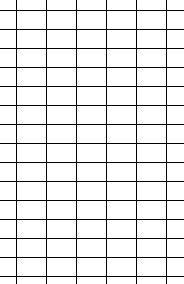
\includegraphics[width=.85\linewidth]{img/BaseGrid}
 \caption{Una semplice griglia strutturata}
 \label{fig:struct_grid}
 \vspace{4ex}
 \end{subfigure}
 \hfill
 %%%%%%%%%%%%%%%%%%%%%%%%%%
  \begin{subfigure}[t]{.48\linewidth}
 \centering
 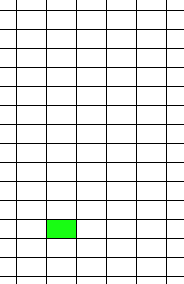
\includegraphics[width=.85\linewidth]{img/CellSelected}
 \caption{Selezioniamo una cella della quale calcoalre i contributi}
 \label{fig:sel_cell}
 \vspace{4ex}
 \end{subfigure}
 
 %%%%%%%%%%%%%%%%%%%%%%%
  \begin{subfigure}[t]{.48\linewidth}
 \centering
 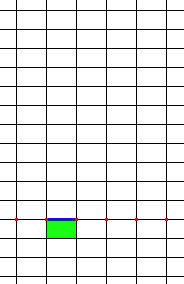
\includegraphics[width=.85\linewidth]{img/Integrating_on_x}
 \caption{Selezioniamo una faccia orizzontale, calcoliamo i contributi della faccia, distribuiamo ai nodi sulla stessa retta}
 \label{fig:integrating_x}
 \vspace{4ex}
 \end{subfigure}
 \hfill
 %%%%%%%%%%%%%%%%%%%%%%%%%%%%
  \begin{subfigure}[t]{.48\linewidth}
 \centering
 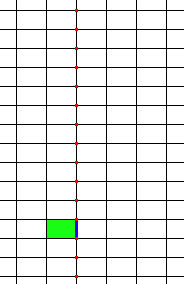
\includegraphics[width=.85\linewidth]{img/Integrating_on_y}
 \caption{Selezioniamo una faccia verticale, calcoliamo i contributi della faccia, distribuiamo ai nodi sulla stessa retta}
 \label{fig:integrating_y}
 \vspace{4ex}
 \end{subfigure}
 \caption{Illustrazione dell'integrazione in \emph{Price}}
 \label{fig:dummy}
\end{figure}


\section{Condizioni al contorno}
Finora non abbiamo menzionato le condizioni al contorno. Trattandosi sempre di condizioni di tipo \emph{dirichlet}, esse vengono imposte una volta assemblato il sistema tramite tecnica di penalizzazione. Esse differiscono leggermente per \emph{price} e \emph{log-price} per via della trasformazione. Osservando le equazioni che dobbiamo trattare, appare chiaro che nel caso monodimensionale le condizioni al bordo da applicare ai nostri problemi siano le seguenti: $$C_h(S_{min},t)=0, \qquad C_h(S_{max},t)=S_{max}-K,$$ per la \emph{call} e:
\begin{equation}
\label{putam_cc}
P_h(S_{min},t)=K-S_{min}, \qquad P_h(S_{max},t)=0,
\end{equation}
per la \emph{put}. Volendo essere pi\`u precisi, tuttavia, imponiamo delle condizioni al bordo con lo \emph{Strike} $K$ scontato, ovvero: $$C_h(S_{min},t)=0, \qquad C_h(S_{max},t)=S_{max}-Ke^{-r(T-t)},$$ per la \emph{call} e: $$P_h(S_{min},t)=Ke^{-r(T-t)}-S_{min}, \qquad P_h(S_{max},t)=0,$$ per la \emph{put}. Questo sconto viene fatto per riportare la quantità monetaria K al tempo $t$ adattandola tramite il tasso d'interesse \emph{risk-free}, in modo da preservare i principi di non arbitraggio. Sarebbe infatti leggermente errato considerare costante nel tempo il valore di un oggetto monetario senza rischio, visto che anch'esso deve rispettare la logica del non arbitraggio.\\Nel caso bidimensionale occorre quindi imporre per ogni nodi di bordo $S_i$: $$C_h(S_i,t)=\max\left(S^1_{max}+S^2_{max}-Ke^{-r(T-t)},0\right)$$per la \emph{call} e: $$P_h(S_i,t)=\max\left(Ke^{-r(T-t)}-S^1_{min}-S^2_{min},0\right),$$ per la \emph{put}.\\
Chiaramente, quando si fa un cambio di variabili per passare al caso \emph{log-price}, è necessario cambiare le condizioni al contorno scrivendole nella nuova variabile. Per esempio per una \emph{call}:
\begin{equation*}
 u_h(x_{min},t)=0, \qquad u_h(x_{max},t)=S_0 e^{x_{max}}-Ke^{-r(T-t)}
\end{equation*}

Analogamente si definiscono le condizioni al bordo per \emph{put} e per il caso bidimensionale.

\section{Il problema con l'ostacolo: il SOR proiettato}
Il metodo pi\`u utilizzato in finanza per risolvere problemi del tipo \eqref{putam1d}  \`e il cosiddetto SOR proiettato, un metodo di risoluzione del sistema lineare iterativo che permette ad ogni iterazione e per ogni punto della griglia di imporre che la soluzione stia sopra all'ostacolo. L'algoritmo, molto semplice da implementare, \`e una variazione del noto metodo SOR, \emph{successive over-relaxation}, derivato dal metodo di \emph{Gauss-Seidel}. Posto quindi: $$z=\frac{1}{a_{ii}}\left(b_i-\sum_{j<i}a_{ij}x_j^{(k+1)}-\sum_{j>i}a_{ij}x_j^{(k)}\right),$$dove $b$ \`e il termine noto, $a$ \`e la matrice e $x^{(k)}$ e $x^{(k+1)}$ sono le soluzione al passo precedente e successivo, al posto della classica iterata $(k+1)$-esima data da: $$x_i^{(k+1)}=x_i^{(k)}+\omega(z-x_i^{(k)}),$$con $0<\omega<2$ fissato, nel SOR proiettato imponiamo: $$x_i^{(k+1)}=\max\left(K-S_i,\quad x_i^{(k)}+\omega(z-x_i^{(k)})\right),$$dove $S_i$ \`e il nodo $i$-esimo della griglia. In questo modo, qualora la soluzione scenda sotto al \emph{payoff}, imponiamo che essa valga esattamente il \emph{payoff} rispettando il vincolo \eqref{putbound}.\\
In questo problema, occorre prestare particolare attenzione alle condizioni al bordo: sebbene la forma sia la stessa, in questo caso non dobbiamo scontare la quantità $K$. Infatti, proprio perché l'opzione può essere esercitata a ogni istante temporale $t\in[0, T]$, il guadagno che si ottiene è pari a $K-S_t$, calcolato usando direttamente lo \emph{strike} $K$. Perci\`o in questo caso la condizione al bordo da imporre \`e nella forma \ref{putam_cc}, ovvero con il prezzo di esercizio non scontato.

\section{\emph{Mesh refinement}}
In questo programma abbiamo implementato anche una funzione che permette di adattare la griglia al problema, in particolare di raffinare o de-raffinare la \emph{mesh} dove ce ne sia bisogno. Per capire in quali punti adattare la griglia abbiamo utilizzato lo stimatore di Kelly, implementato direttamente nella libreria \textsf{deal.ii}. Esso stima l'errore soltanto per l'equazione generalizzata di Poisson: $$-\nabla\left(a(x)\nabla u\right)=f,$$tuttavia \`e uno stimatore utilizzato spesso perch\'e permette di stimare la differenza fra i gradienti della soluzione in due celle vicine. Qualora questa differenza sia troppo grande, ovvero la soluzione cambi molto inclinazione fra celle vicine, allora \`e necessario raffinare la griglia. Se invece la differenza fra i gradienti \`e nulla o molto piccola, allora \`e possibile de-raffinare la \emph{mesh}.\\
A causa dell'algoritmo usato per il calcolo delle parti integrali, il \emph{mesh refinement} non è compatibile con la trasformazione \emph{price} nel caso bidiminesionale. Infatti, se per esempio una cella venisse raffinata, si verrebbe a creare un nodo che appartiene a un segmento lungo l'asse $x$ (e a uno lungo l'asse $y$) ma che esiste solo all'interno della cella raffinata, e non su tutto il dominio. In tal caso, a quel nodo si sommerebbero i contributi solo di quella cella e non di tutto $[S_{min},S_{max}]$, il che porterebbe a un errore concettuale. Per questo motivo, il \emph{mesh refinement} della PIDE bidimensionale in \emph{price} \`e disattivato. Nella trasformazione \emph{log-price} non vi sono invece problemi, dato che il metodo implementato funziona su una griglia qualunque.

\chapter{Pacchetti usati}
\section{\textsf{deal.ii}}
\textsf{deal.ii} \`e una libreria scritta in c++ che permette di risolvere tramite metodi a elementi finiti per una grande variet\`a di problemi alle derivate parziali. Fra i suoi maggiori pregi, oltre alla presenza di elementi finiti di ogni ordine, troviamo la grande scalabilit\`a (\`e stato infatti provato che questa libreria riesce a scalare fino a 16.000 processori), la possibilit\`a di interfacciarsi con molte librerie come \textsf{PETSc}, \textsf{Trilinos}, \textsf{METIS}, \textsf{BLAS}, \textsf{LAPACK}, e la vastit\`a e la precisione della documentazione. Soffermandoci un attimo su questo ultimo punto, vorremmo proprio sottolineare la presenza di una documentazione (quasi) sempre precisa e ben organizzata. Oltre a questa, ci sono inoltre 51 tutorial che insegnano a utilizzare la libreria dalla semplice creazione di una \emph{mesh} bidimensionale fino alla risoluzione di problemi iperbolici di meccanica non lineare in 3d con \emph{mesh refinement}. Per scrivere il nostro codice abbiamo sfruttato molto la massiccia documentazione della libreria, e siamo stati quasi sempre in grado di trovare le funzioni che facevano al caso nostro. In una occasione tuttavia non siamo riusciti a trovare un metodo e abbiamo deciso di scrivere sul gruppo \url{https://groups.google.com/forum/#!forum/dealii}, ottenendo una risposta precisa in breve tempo.\\%Tornando alla parte implementativa, per risolvere i sistemi lineari, abbiamo sfruttato l'integrazione di \textsf{deal.ii} con la libreria di solutori diretti per matrici sparse asimmetriche UMFPACK, come consigliato in alcuni dei tutorial.\\
%In generale, un problema a elementi finiti viene affrontato in \textsf{deal.ii} creando una triangolazione (\textsf{Triangulation}), un \emph{handler} dei gradi di libert\'a (\textsf{DoF\_Handler}) e un oggetto elementi finiti (\textsf{FE\_Q} per esempio). Si costruiscono le varie matrici del sistema e si usano i \emph{solver} integrati per risolvere il sistema.
In definitiva, la libreria \textsf{deal.ii} si presenta come un prodotto solido e con una curva di apprendimento molto morbida all'inizio, ma che necessita un po' pi\'u di sforzo se si vogliono utilizzare funzionalit\`a meno comuni.

\section{\textsf{Cmake}}
La libreria \textsf{deal.ii} utilizza \textsf{Cmake} per compilare i codici dei tutorial. Perci\`o anche noi abbiamo utilizzato questo \emph{tool}. In particolare, in un qualsiasi file \textsf{CMakeLists.txt} come quelli forniti da \textsf{deal.ii} occorre aggiungere tutti i file sorgente, scrivere il nome dell'eseguibile desiderato e il \textsf{CMake} crea da solo il \textsf{Makefile} specificando dove si trovano gli \emph{header file} da includere e le librerie di \textsf{deal.ii} da linkare. Utilizzando due sistemi operativi diversi, il \textsf{CMake} \`e stato molto utile per poter lavorare sui codici senza avere problemi di portabilit\`a che pu\`o avere il semplice \textsf{Makefile}. Inoltre, siccome abbiamo utilizzato nel nostro codice \textsf{OpenMP} e il \textsf{CMakeLists.txt} di \textsf{deal.ii} non lo prevede, abbiamo aggiunto la ricerca del pacchetto \textsf{OpenMP} nel modo seguente:
\begin{lstlisting}
find_package(OpenMP)
if (OPENMP_FOUND)
    set (CMAKE$\_$C$\_$FLAGS "$\$\{$CMAKE$\_$C$\_$FLAGS$\}$
	$\$\{$OpenMP$\_$C$\_$FLAGS$\}$")
    set (CMAKE$\_$CXX$\_$FLAGS "$\$\{$CMAKE$\_$CXX$\_$FLAGS$\}$
	$\$\{$OpenMP$\_$CXX$\_$FLAGS$\}$")
endif()
\end{lstlisting}
in modo che, se il \textsf{CMake} trova \textsf{OpenMP}, aggiunge il \emph{flag} \textsf{-fopenmp} al compilatore, altrimenti non aggiunge nulla.\\
\iffalse
Abbiamo infine aggiunto:
\begin{lstlisting}
FIND_PACKAGE(Doxygen)
IF(NOT DOXYGEN_FOUND)
	MESSAGE(FATAL ERROR "Doxygen not found")
ENDIF()
CONFIGURE_FILE(doxy-config \@ ONLY IMMEDIATE)
ADD_CUSTOM_TARGET(doc
	COMMAND $\$\{$DOXYGEN_EXECUTABLE$\}$ doxy-config )
\end{lstlisting}
in modo da creare il \emph{target} \textsf{doc} che generi la documentazione con \textsf{Doxygen}.
\fi
\section{GitHub}
Durante lo sviluppo di questo progetto, abbiamo sempre utilizzato il sistema di controllo di versioni Git e il servizio di \emph{web hosting} GitHub per lo sviluppo di progetti software. Abbiamo quindi creato una \emph{repository} remota all'indirizzo \url{https://github.com/NTFrs/pacs_proj}. L'uso di git ci ha permesso di lavorare in contemporanea sul progetto senza doverci preoccupare di fare cambiamenti allo stesso file, anche attraverso l'uso di diversi \emph{branch}.
\begin{figure}[!htb]
 \begin{center}
 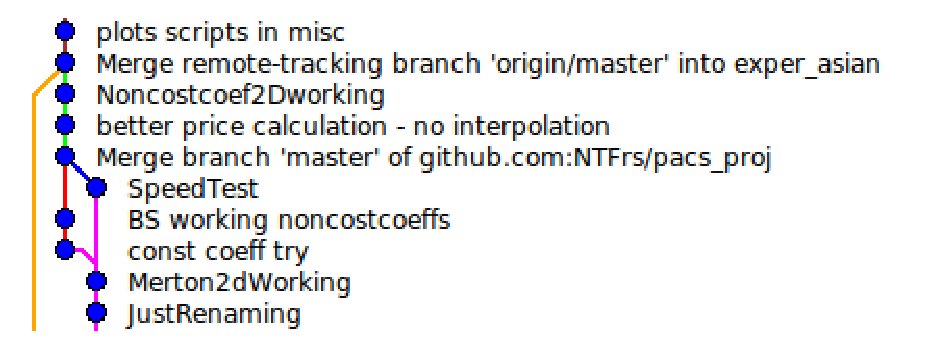
\includegraphics[width=8cm]{img/Git.eps}
 \caption{Cammino di alcuni \emph{branch} sui quali abbiamo lavorato. Immagine tratta da \textsf{gitk}.}
 \label{fig:gitk}
 \end{center}
\end{figure}
\section{Profilers e Memory Checkers: \textsf{gprof} e \textsf{valgrind}}
Durante la scrittura dei codici finali, abbiamo notato che alcune parti del programma erano più lente rispetto a implementazioni fatte precedentemente. L'utilizzo del \emph{profiler} \textsf{gprof} ci ha permesso di analizzare e ristrutturare quelle parti ottenendo uno \emph{speedup} considerevole, anche rispetto ai codici antecedenti. In particolare, il calcolo dell'integrale con la trasformazione \emph{price} non era molto veloce, e tramite il \emph{profiler} abbiamo scoperto che una delle funzioni di \textsf{deal.ii} di accesso agli elementi della griglia era particolarmente lenta. Abbiamo quindi cercato di ridurre quanto possibile il numero di chiamate ad essa.\\
Abbiamo anche analizzato il codice con l'uso di \textsf{valgrind} e usando i seguenti \emph{tool}:
\begin{itemize}
 \item \textsf{callgrind}: nel caso \emph{log-price}, eravamo interessati a sapere quanto la parte \textsf{compute\_J()} incidesse sul programma per valutare l'effetto della parallelizzazione. Purtroppo, \textsf{gprof} non riesce a riconoscere bene la successione di chiamate di funzioni (in particolare alcune interne a \textsf{deal.ii}) e quindi abbiamo utilizzato il tool \textsf{callgrind} di \textsf{valgrind} insieme al visualizzatore \textsf{KCacheGrind} (o \textsf{QCacheGrind}), ottenendo un'analisi migliore. La figura \ref{fig:callgraph} riporta la parte del \emph{call graph} a cui eravamo interessati. Fra i programmi forniti si può trovare \textsf{profiled} che implementa il test, cos\`i come il file ottenuto in seguito al profiling.
 \item \textsf{memcheck}: abbiamo inoltre analizzato i nostri programmi alla ricerca di \emph{memory leaks}, notando un comportamento un po' strano di \textsf{valgrind}: l'output del programma afferma che non ci sono problemi di memoria, ma \`e possibile che ci sia un \emph{leak} di 792 byte. Questo valore rimane costante in ogni programma testato, anche allocando due o pi\`u oggetti Opzione, e la lista di chiamate a funzione stampata da \textsf{valgrind} indica che il problema si trova all'interno della funzione che esegue il prodotto matrice-vettore di \textsf{deal.ii}. Per questo motivo riteniamo che \textsf{valgrind} non capisca cosa succeda in quella funzione e ritenga che ci possa essere un \emph{memory leak}. A scanso di equivoci, abbiamo anche analizzato i programmi con un \emph{tool} di Xcode che controlla l'uso della memoria, e quest'ultimo non ha evidenziato alcun problema.
\end{itemize}
\begin{figure}[!htb]
 \makebox[\textwidth][c]{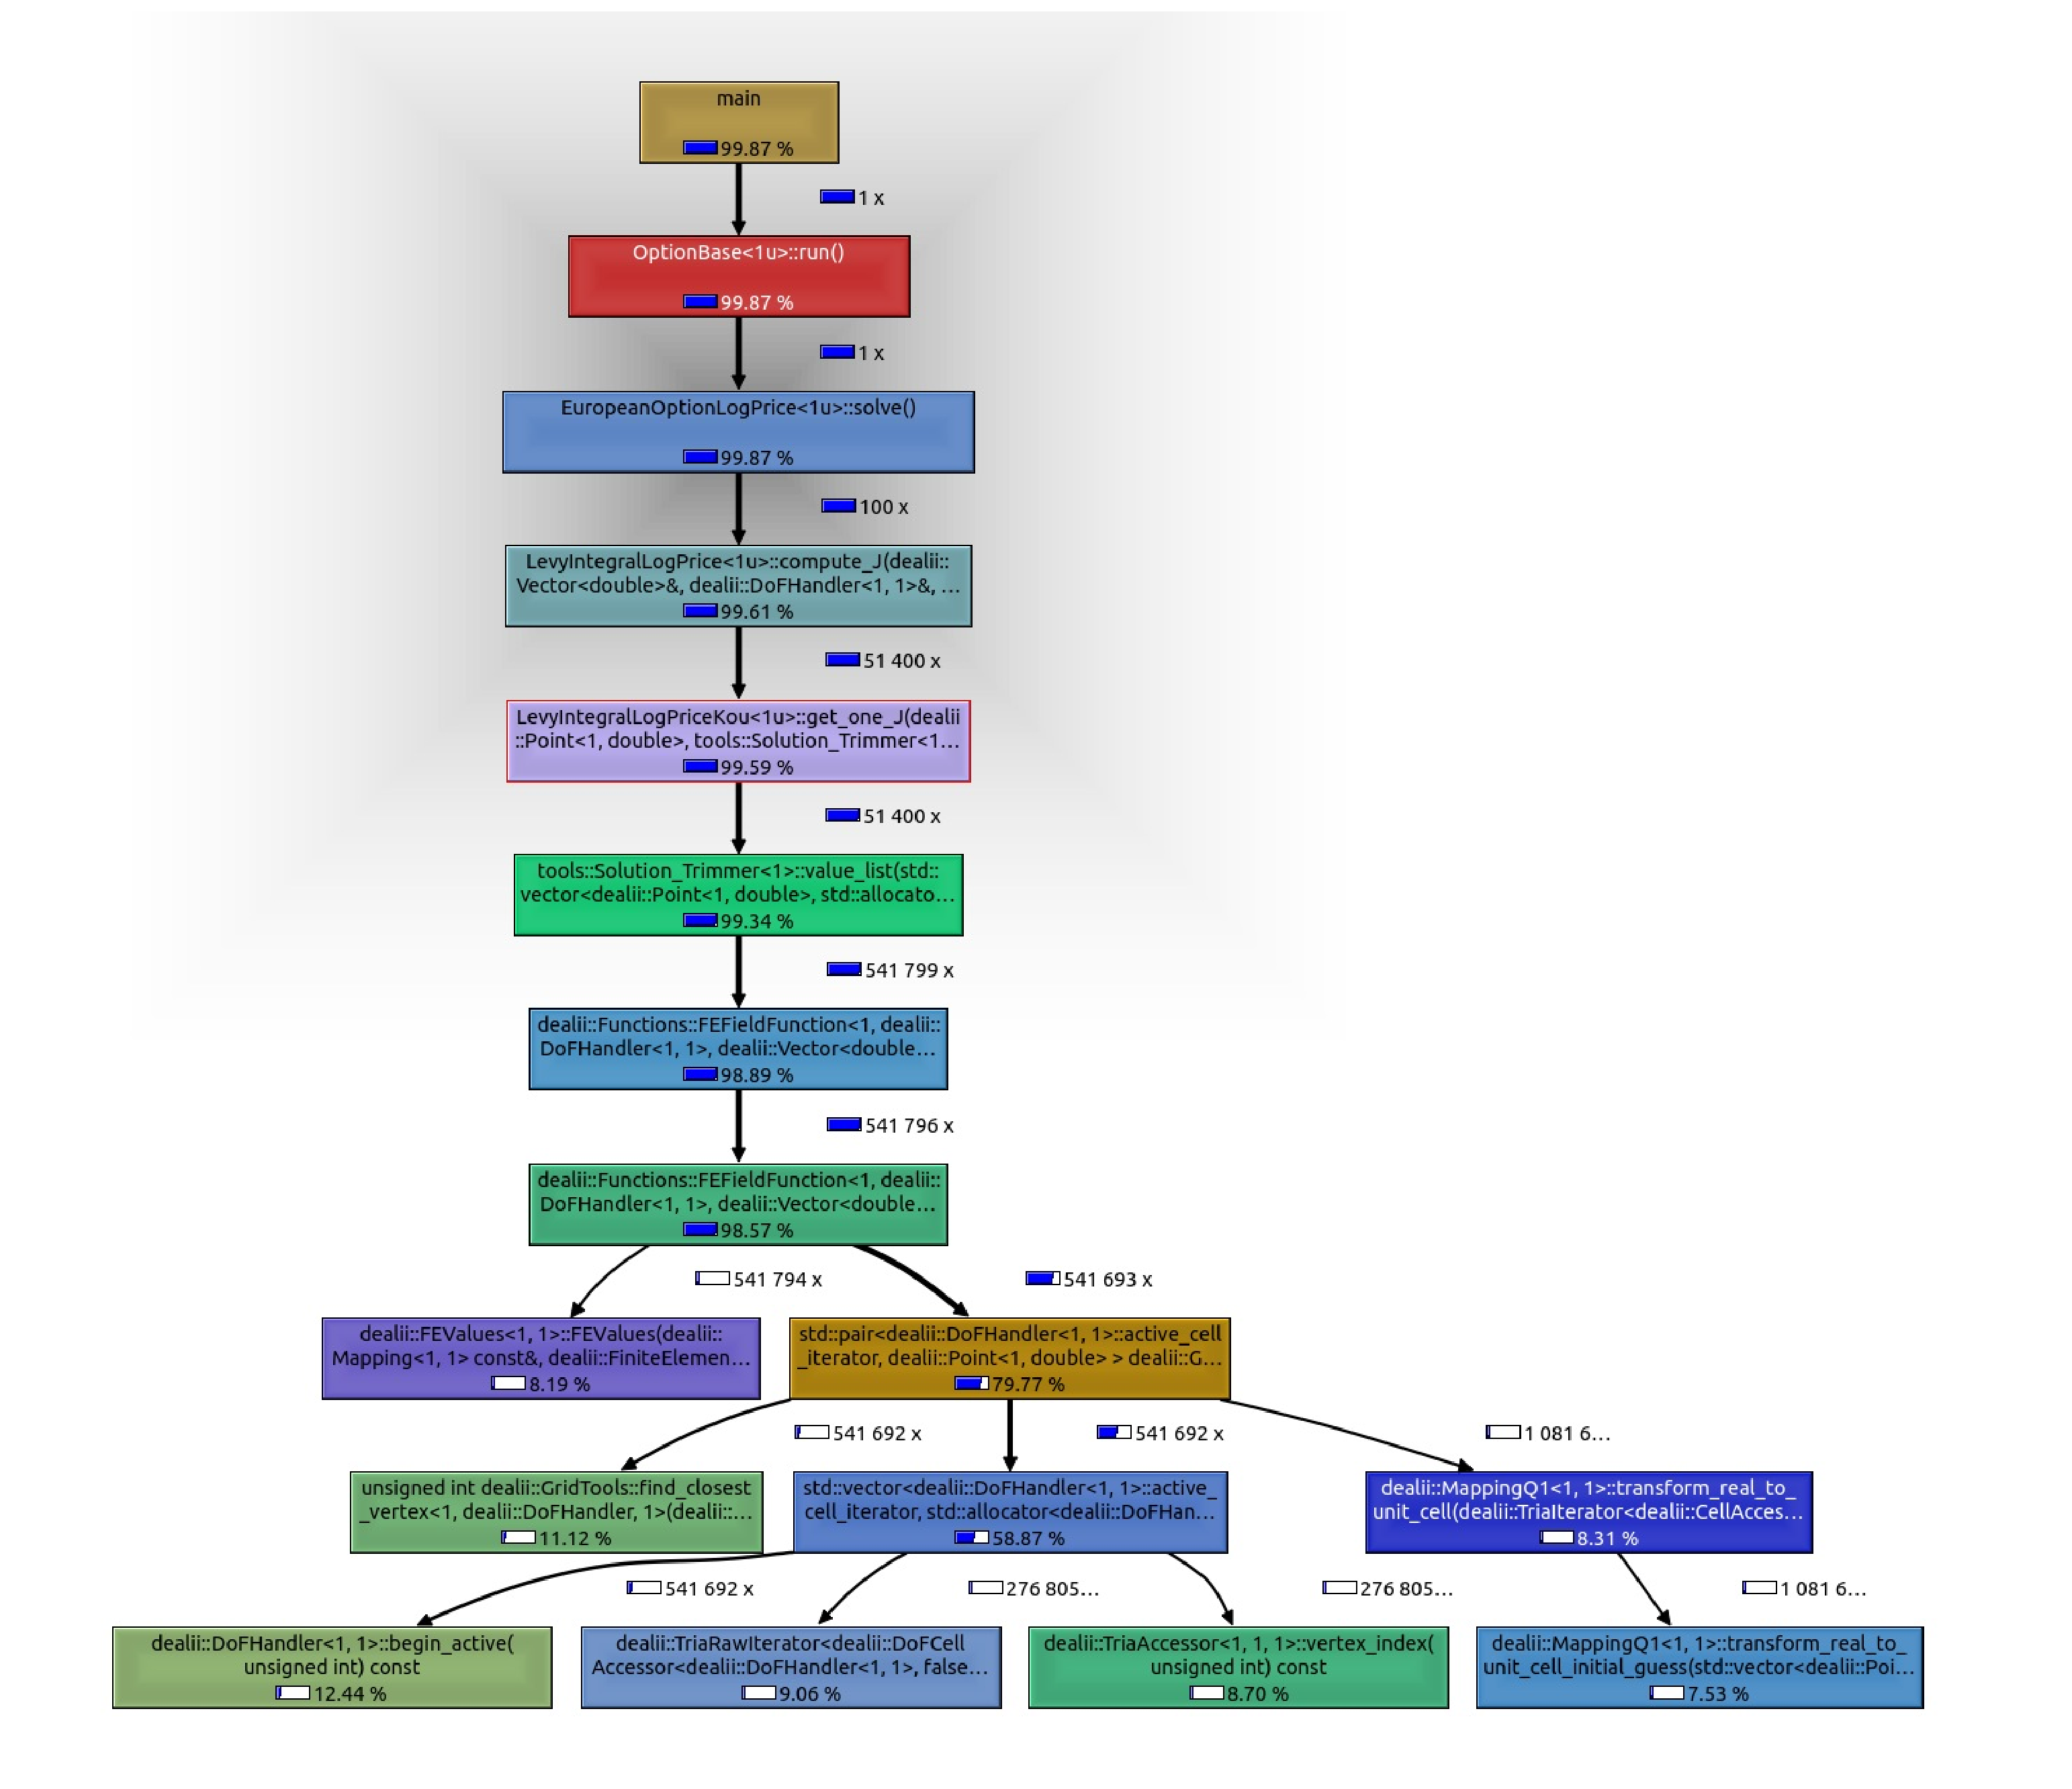
\includegraphics[width=1.4\textwidth]{img/callgraph.eps}}
 \caption{Call Graph generato da \textsf{KCacheGrind} con i pesi relativi delle funzioni per un'opzione con trasformazione \emph{log-price} monodimensionale. Le funzioni con un costo relativo basso non sono mostrate.}
\label{fig:callgraph}
 \end{figure}
\section{\textsf{Doxygen}}
Tutto il codice \`e commentato con il \emph{lexical-scanner} \textsf{Doxygen}, molto semplice da utilizzare. 
\section{Quadrature Rules}
Per il calcolo degli integrali con nodi di Laguerre e Hermite, abbiamo utilizzato una piccola libreria di funzioni utilizzata durante uno dei laboratori del corso, disponibile sul sito \url{http://people.sc.fsu.edu/~jburkardt/cpp_src/laguerre_rule/laguerre_rule.cpp} e distribuita sotto la licenza GNU LGPL. Si tratta di un insieme di funzioni scritte in C che permettono di calcolare nodi di integrazione di diverso tipo: oltre a quelli di nostro interesse, Chebyshev, Jacobi, esponenziali, razionali e altri.
\section{\textsf{astyle}}
Abbiamo infine utilizzato un piccolo programma disponibile al sito \url{http://astyle.sourceforge.net/} che permette di formattare automaticamente il codice, in modo da avere un \emph{layout} uniforme in tutti i file sorgente.
\chapter{Codice}
\section{Introduzione}
In questo capitolo descriviamo come il problema \`e stato implementato da un punto di vista computazionale, elencando le varie classi scritte e le loro caratteristiche. Inizialmente mostriamo delle piccole classi che si occupano di gestire i parametri dei modelli e le loro densit\`a. Nella seconda sezione descriviamo gli oggetti opzione che costruiscono il sistema per risolvere il problema a elementi finiti in una e due dimensioni. Questi oggetti utilizzano poi le funzioni di altri oggetti, \textsf{LevyIntegral}, per il calcolo della parte integrale. Successivamente, descriviamo brevemente la \emph{Factory} che abbiamo scritto per istanziare gli oggetti opzione e infine spieghiamo brevemente le linee guida per utilizzare questa libreria.
\section{Classi per i Modelli}
Il primo blocco di classi scritto nel nostro codice permette di gestire i vari modelli utilizzati per descrivere la dinamica del sottostante, in particolare i modelli di \emph{Black\&Scholes}, \emph{Kou} e \emph{Merton}. Abbiamo quindi deciso di scrivere una classe astratta \textsf{Model}, che contenga i parametri comuni ai diversi oggetti e tutti i metodi utilizzati. Come possiamo osservare in figura \ref{modelbase}, da questa classe ereditano in maniera pubblica le tre classi modello non pi\`u astratte, ed esse contengono i parametri propri di ogni modello.
\begin{figure}[h!]
\begin{center}
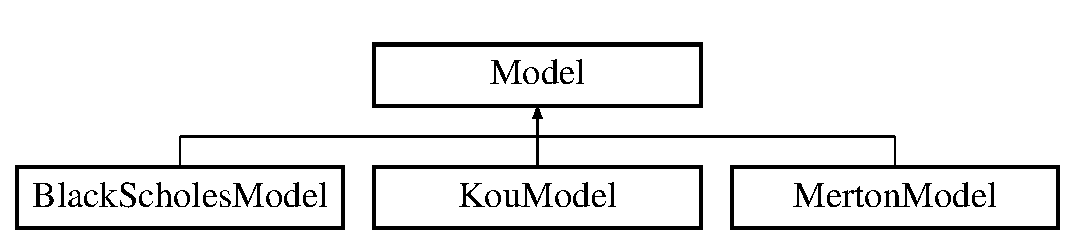
\includegraphics[width=12cm]{img/classModel.eps}
\label{modelbase}
\caption{Gerarchia delle classi modello}
\end{center}
\end{figure}
\section{Classi per Opzioni}
Le classi per Opzioni sono la componente centrale del programma e permettono di istanziare e gestire il problema di differenziale. Sono state scritte secondo le linee guida della libreria \textsf{deal.ii}. Le loro caratteristiche principali sono dunque le seguenti:
\begin{itemize}
\item {come tutte le classi presentate nei \emph{tutorial} di \textsf{deal.ii}, anche le nostre hanno la dimensione (nel nostro caso 1 o 2) come parametro \emph{template}}
\item {i pi\`u importanti metodi privati (o meglio, protetti) e pubblici dell'oggetto Opzione sono i seguenti:}
\begin{enumerate}
\item \textsf{virtual void setup\_system()};
\item \textsf{virtual void make\_grid()};
\item \textsf{virtual void assemble\_system()};
\item \textsf{virtual void refine\_grid()};
\item \textsf{virtual void setup\_integral()}, aggiunto da noi per allocare le classi che si occupano della parte integrale;
\item \textsf{virtual void solve()}, metodo che risolve il sistema lineare;
\item \textsf{virtual void run()}, metodo pubblico che chiama in ordine tutti i precedenti e calcola la soluzione.
\end{enumerate}
\end{itemize}
A questi metodi sono state aggiunte altre funzioni che permettono di impostare alcune variabili del problema.\\Per quanto riguarda la struttura gerarchica di queste classi, poich\'e il nostro scopo \`e calcolare il prezzo di opzioni europee e americane con trasformazioni \emph{price} e \emph{log-price} e poich\'e alcuni metodi sono comuni ai diversi problemi e alle diverse trasformazioni, abbiamo deciso di sfruttare l'ereditariet\`a delle classi permessa dal c++ facendo chiamare al programma per ogni problema i metodi opportuni.
\begin{figure}[h!]
\begin{center}
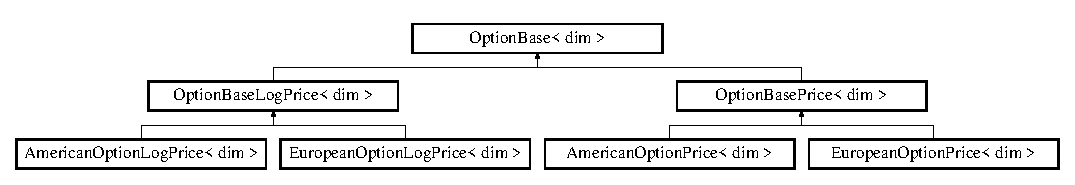
\includegraphics[width=12cm]{img/classOptionBase.eps}
\caption{Gerarchia delle classi opzione}
\label{optionbase}
\end{center}
\end{figure}
\subsection{\textsf{OptionBase$<$dim$>$}}
Entrando pi\`u nel dettaglio, come possiamo osservare nella figura \ref{optionbase}, abbiamo scritto una classe base \textsf{OptionBase$<$dim$>$} astratta, nel cui campo \textsf{protected} sono contenute tutte le variabili del problema, quali gli oggetti \textsf{dealii::FE\_Q$<$dim$>$}, \textsf{dealii::DoFHandler$<$dim$>$} e \textsf{dealii::Triangulation$<$dim$>$} che gestiscono elementi finiti, gradi di libert\`a e \emph{mesh}, gli oggetti che memorizzano le matrici e i \textsf{dealii::Vector$<$double$>$} della soluzione e del \emph{right hand side}. Per quanto riguarda l'oggetto che gestisce la matrice di sistema, poich\'e uno dei nostri problemi necessita di un \emph{solver} particolare non presente nella libreria utilizzata, ovvero il PSOR, abbiamo deciso di scrivere un piccolo decoratore. Questo oggetto, \textsf{dealii::SparseMatrix\_PSOR$<$double, dim$>$} eredita pubblicamente da \textsf{dealii::SparseMatrix$<$double$>$} e aggiunge un metodo che risolva il problema con l'ostacolo. Come sappiamo, i costruttori non vengono ereditati, perci\`o sono stati riscritti in modo che chiamino i costruttori della classe base. Inoltre, siccome i metodi di \textsf{dealii::SparseMatrix$<$double$>$} non sono \textsf{virtual}, abbiamo aggiunto all'interno della nostra classe:
\begin{lstlisting}
// SparseMatrix methods
using dealii::SparseMatrix<number>::reinit;
using dealii::SparseMatrix<number>::add;
\end{lstlisting}
in modo che il compilatore capisca che deve utilizzare i metodi \textsf{reinit} e \textsf{add} di \textsf{dealii::SparseMatrix$<$double$>$}.\\\\Per quanto riguarda invece i costruttori della classe Opzione, essi sono specializzati per $1$ e $2$ dimensioni. In particolare, il costruttore $1$d prende un puntatore alla classe base \textsf{Model} e i vari parametri dell'opzione (quali tasso di interesse, scadenza e \emph{strike}), mentre il costruttore $2$d prende due puntatori a due oggetti \textsf{Model} e i vari dati dell'opzione. I costruttori si occupano di creare gli oggetti relativi agli elementi finiti e li collegano alla \emph{mesh}. I metodi invece che implementiamo qui sono \textsf{void setup\_system()} che si occupa di creare lo \emph{sparsity pattern} delle matrici e inizializzarle e \textsf{void refine\_grid()} che, tramite lo stimatore di \emph{Kelly}, esegue un adattamento della griglia.
\subsection{\textsf{OptionBasePrice$<$dim$>$} e \textsf{OptionBaseLogPrice$<$dim$>$}}
Le classi \textsf{OptionBasePrice$<$dim$>$} e \textsf{OptionBaseLogPrice$<$dim$>$}, anch'esse astratte, ereditano da \textsf{OptionBase$<$dim$>$} e definiscono parte dei metodi descritti nell'introduzione. Le due classi implementano la funzione \textsf{void make\_grid()} che crea la \emph{mesh} nei casi \emph{price} e \emph{log-price}, ovvero con le opportune trasformazioni, il metodo \textsf{void assemble\_system()} che integra gli elementi finiti e costruisce le matrici di sistema in 1d e 2d e il metodo \textsf{double get\_price()}, che valuta la soluzione nel punto $x=(0,0)$ per il \emph{log-price} e $\underline{S}=(S_0^1, S_0^2)$ per il \emph{price}, ovvero che restituisce il prezzo dell'opzione. Infine, la classe \textsf{OptionBasePrice$<$dim$>$} implementa qui il metodo \textsf{void setup\_integral()} che istanzia dinamicamente un oggetto di tipo \textsf{LevyIntegral}, che si occupa di calcolare la parte integrale. \textsf{OptionBaseLogPrice$<$dim$>$} invece non lo istanzia qui ma nel "livello" di ereditarier\`a successivo poich\'e con questa trasformazione occorre conoscere le condizioni al bordo per poter calcolare l'integrale.
\subsection{\textsf{AmericanOption$<$dim$>$} e \textsf{EuropeanOption$<$dim$>$}}
Queste quattro classi alla base della piramide sono gli oggetti utilizzati per risolvere i vari problemi. Essi implementano le varie funzioni \textsf{void solve()} che risolvono il sistema lineare. In primo luogo quindi viene proiettata sulla \emph{mesh} la condizione finale (ovviamente diversa fra \emph{put} e \emph{call}, \emph{price} e \emph{log-price}) e successivamente parte il ciclo temporale che applica le condizioni al bordo, calcola il vettore integral $J$ se il modello non \`e \emph{Black\&Scholes} e risolve il sistema. Per quanto riguarda quest'ultimo passaggio, per l'europea abbiamo utilizzato un \emph{solver} usato da \textsf{deal.ii}, ovvero \textsf{SparseDirectUMFPACK}, mentre per l'americana usiamo il \emph{solver} scritto all'interno del decoratore di \textsf{dealii::SparseMatrix$<$double$>$}.

%%%%%%%%%%%%%%%%%%%%%%%%%%%%%%%%%%%%%%%%%%%%%%%%%%%%%%%%%%%%%%%%%%%%%%
\section{Classi per il calcolo degli integrali}
Per il calcolo della parte integrale dell'equazione, ossia la quadratura di $\hat{\alpha}$ e il calcolo dei vettori $J_i$ ad ogni iterazione temporale, sono state costruite una serie di classi. Tali classi ereditano da una classe comune di base che definisce l'interfaccia. Usando questo schema con ereditarietà (mostrato in figura \ref{fig:levybase}) siamo riusciti a mantenere un'interfaccia comune, pur allocando classi specifiche per modelli specifici. Cos\`i come le classi opzione, anche queste classi sono \emph{templatizzate} sulla dimensione, poiché il calcolo dell'integrale può essere anche molto diverso fra una e due dimensioni.
\begin{figure}[h!]
\begin{center}
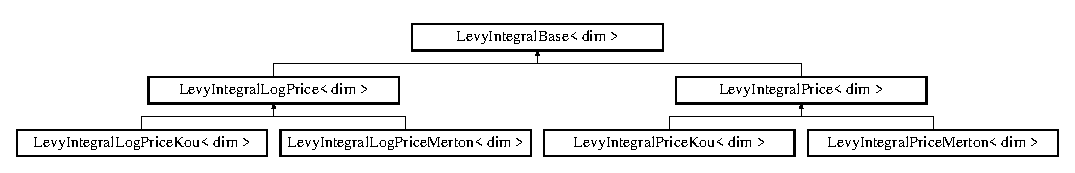
\includegraphics[width=12cm]{img/classLevyIntegralBase.eps}
\caption{Gerarchia delle classi LevyIntegral}
\label{fig:levybase}
\end{center}
\end{figure}
\subsection{\textsf{LevyIntegralBase$<$dim$>$}}
Questa classe astratta definisce un'interfaccia condivisa e sfruttata da tutte le classi per la quadratura dell'integrale e implementa alcuni metodi di base che possono essere utili alle classi figlie.\\
I due metodi \emph{core} della classe sono \textsf{void compute\_alpha()}, che calcola il valore degli $\hat{\alpha}_i$, e \textsf{void compute\_J()}, che calcola il valore della parte integrale da usare nell'\emph{rhs}. Osserviamo inoltre che questa classe base definisce già una funzione che calcola $\hat{\alpha}_i$ in modo generico, ossia con una quadratura composita con nodi di Gauss, e che funziona dunque con qualsiasi modello.

\subsection{\textsf{LevyIntegralPrice$<$dim$>$} e \textsf{LevyIntegralLogPrice$<$dim$>$}}
La seconda parte dell'integrale, ossia i vettori $J_i$, è totalmente diversa a seconda che si utilizzi la trasformazione \emph{price} o \emph{log-price}. Per questo motivo abbiamo scritto due classi che ereditano da \textsf{LevyIntegralBase$<$dim$>$}. Siccome sono ancora generiche e non sono specializzate su modelli specifici, ereditano dalla classe base il metodo \textsf{compute\_alpha()}, che calcola $\hat{\alpha}_i$ per un qualsiasi modello.\\\\La classe \textsf{LevyIntegralLogPrice$<$dim$>$} implementa il metodo \textsf{void compute\_J()} per la forma \emph{log-price}, che risulta essere pi\`u semplice ma allo stesso tempo più lento rispetto al metodo utilizzato dalla trasfomazione \emph{price}. Sia in una che in due dimensioni (e potenzialmente in più), il calcolo di $J_i$ viene svolto ciclando su tutti i nodi della griglia e calcolando in ciascuno il valore dell'integrale. Per fare questo, utilizziamo la classe ausiliaria \textsf{Solution\_Trimmer$<$dim$>$} e il metodo \textsf{get\_one\_J}. \textsf{Solution\_Trimmer$<$dim$>$} è sostanzialmente un funtore che, inizializzato con la soluzione e la mappatura dei gradi di libertà di \textsf{deal.ii} (cio\`e, il \textsf{DoFHandler}) agisce diversamente a seconda che il punto stia dentro o fuori dal dominio. Nel primo caso chiama una funzione di \textsf{deal.ii} che individua in che cella si trova il nodo e restituisce il valore della funzione in tale punto, nel secondo caso impone il valore al bordo. La parte computazionalmente costosa è appunto la valutazione in un punto interno al dominio, poiché le funzioni della libreria devono individuare in quale cella si trova quel punto (ricordiamo qui che la funzione incognita va valutata nel punto $y_l+x_i$, dove $y_l$ sono i punti di quadratura e $x_i$ il nodo attuale, quindi per ogni nodo in punti diversi). Una volta ottenuto il valore della soluzione nel punto (sia esso dentro o fuori dal dominio) è possibile effettuare la quadratura dell'integrale. Il calcolo del contributo del nodo $i$ a $J_i$ viene fatto dal metodo \textsf{get\_one\_J}. Questa struttura è pensata per poter utilizzare un altro tipo di quadratura nelle classi figlie, ridefinendo solo \textsf{get\_one\_J}. A questo livello, non essendo specificato alcun modello, utilizziamo una quadratura generica (cio\`e i soliti nodi di Gauss). Per ridurre le operazioni di copia di vettori, \textsf{compute\_J} è specializzata sulla dimensione, ma i cambiamenti fra una e due dimensioni sono quasi nulli.
\\\\
La classe \textsf{LevyIntegralPrice$<$dim$>$}, invece, implementa \textsf{compute\_J()} specializzando il metodo sul parametro \emph{template}, ottenendo funzioni sostanzialmente diverse. Infatti, come già spiegato nella sezione \ref{sec:Price}, i metodi utilizzati per calcolare la parte integrale $J$ sono fondamentalmente diversi a seconda della dimensione.\\In una dimensione, per ogni nodo della griglia, occorre integrare scorrendo tutte le celle e calcolandone il contributo. In due dimensioni, il contributo a $J_1$ nel nodo $S_i$ è calcolato sulla retta monodimensionale parallela all'asse delle ascisse, mentre il contributo a $J_2$ è calcolato lungo la retta parallela all'asse delle ordinate. Quindi, per ogni nodo, il metodo scorre le facce di tutte le celle della griglia, e, se la faccia sta sulla retta passante per il nodo corrente, ne calcola il contributo. Sebbene questa sia una procedura complicata, richieda una griglia strutturata e richieda che tutti i nodi vengano visitati ma solo alcuni presi in considerazione, essa risulta più rapida rispetto al calcolo con il metodo \emph{log-price}. Infatti, con questo secondo metodo, la soluzione viene valutata nei nodi di quadratura che cadono sulla faccia attuale, quindi le funzioni della libreria conoscono la cella in cui cadono i nodi di quadratura e restituiscono velocemente il valore, senza dover cercare il nodo su tutta la griglia.

\subsection{Le classi figlie per modelli specifici}

Come si nota in figura \ref{fig:levybase}, esistono poi delle classi derivate da \textsf{LevyIntegralPrice $<$dim$>$} e \textsf{LevyIntegralLogPrice$<$dim$>$}. Esse implementano di nuovo i metodi per il calcolo delle parti integrali con dei nodi di quadratura specifici per i vari modelli. In particolare \textsf{LevyIntegralPriceKou$<$dim$>$} e \textsf{LevyIntegralPriceMerton$<$dim$>$} implementano solo la funzione \textsf{void compute\_alpha()} utilizzando rispettivamente nodi di Laguerre e di Hermite, poich\'e grazie alla trasformazione $y=Se^y$, le densit\`a contro cui integriamo non sono pi\`u esponenziali o gaussiane. Le classi \textsf{LevyIntegralLogPriceKou$<$dim$>$} e {LevyIntegralLogPriceMerton$<$dim$>$}, invece, oltre a implementare di nuovo \textsf{void compute\_alpha()} con i nodi specifici, implementano pure \textsf{get\_one\_J} sfruttando le potenzialit\`a dei nodi specializzati sui modelli. Nel caso si vogliano aggiungere altri modelli, questo design permette di creare nuove classi specifiche che ereditano dal secondo livello, permettendo all'utente di modificare solo piccole parti.

\section{\emph{Factory}}
Data la complessit\`a strutturale delle classi Opzione, abbiamo deciso di utilizzare il \emph{design pattern} della \emph{factory} descritta in \cite{gamma1994design}, altrimenti noto come costruttore virtuale, per permettere a un qualsiasi utente di istanziare l'oggetto giusto per il suo problema. Abbiamo quindi creato una classe, \textsf{Factory} che ha costruttore di default, costruttore di copia e operatore di copia privati, perci\`o non \`e possibile istanziare la classe, e abbiamo scritto il seguente metodo:
\begin{lstlisting}
static Factory * instance()
        {
                static Factory instance;
                return &instance;
        }
\end{lstlisting}
Questa funzione permette di istanziare uno e un solo oggetto della classe \textsf{Factory}, che \`e quindi un \emph{singleton}. Oltre a questo metodo, abbiamo due funzioni \textsf{std::unique\_ptr$<$OptionBase$<$dim$>$ $>$ create(...)} con il parametro \textsf{dim} specializzato su una e due dimensioni che prendono come argomenti il tipo di opzione, europea o americana, \emph{put} o \emph{call}, il tipo di trasformazione, i modelli dei sottostanti e i vari parametri dell'opzione.
\section{Come utilizzare la libreria}
Sfruttando la \emph{factory} di cui abbiamo appena parlato, utilizzare questa libreria \`e molto semplice:
\begin{itemize}
\item la prima cosa da fare \`e creare un oggetto di tipo \textsf{Model}, introducendo parametri come il valore del sottostante, la sua volatilit\`a e l'intensit\`a dei salti, nel caso di un modello di L\'evy,
\begin{lstlisting}
BlackScholesModel model(95., 0.120381);
\end{lstlisting}
\item dopodich\'e, utilizzando la \emph{factory}, si stabilisce che tipo di opzione istanziare, europea o americana, \emph{put} o \emph{call}, con trasformazione \emph{price} o \emph{log-price}, e si passano i parametri del contratto e di mercato, quali tasso di interesse, scadenza del contratto, prezzo di esercizio, e i parametri di discretizzazione,
\begin{lstlisting}
auto foo=
Factory::instance()->create(ExerciseType::EU,
OptionType::Put,
Transformation::Price,
model.get_pointer(),
0.0367, 1., 90., 12, 250);
\end{lstlisting}
\item poi, dopo aver settato alcuni parametri e flag a discrezione dell'utente, occorre chiamare la funzione:
\begin{lstlisting}
foo->run();
\end{lstlisting}
che crea il sistema e lo risolve.
\item infine, per stampare il prezzo del titolo finanziario,
\begin{lstlisting}
std::cout<<"The price of the option is "<<foo->get_price()<<std::endl;
\end{lstlisting}
\end{itemize}
\chapter{Risultati}
In questo capitolo riportiamo e commentiamo i risultati ottenuti tramite la nostra libreria. In particolare, analizzeremo nel dettaglio i vari output ottenuti dai programmi \textsf{test} contenuti a titolo esplicativo nel nostro codice. Tutti i risultati seguenti sono stati ottenuti su un computer con un processore \emph{intel i5} quad-core, con 4GB di memoria RAM e la versione 8.1.0 di \textsf{deal.ii}.
\section{\textsf{test-1}}
In questo primo semplice programma, abbiamo calcolato il prezzo di opzioni europee il cui sottostante evolve secondo un classico modello di \emph{Black\&Scholes}, ovvero l'equazione da risolvere \`e la solo PDE, senza parte integrale. I risultati ottenuti sono illustrati nella tabella \ref{test1-1}.
\begin{table}[htp!]
\begin{center}
\begin{tabular}{| l | l | l | l | l | l |}
\hline
Dimensione & Trasformazione & Griglia & Timesteps & Prezzo & Tempo \\ \hline
1 & \emph{price} & 4096 & 250 & 1.42046\officialeuro & 1.36864s \\ \hline
1 & \emph{log-price} & 4096 & 250 & 1.42046\officialeuro & 1.38591s \\ \hline
2 & \emph{price} & 16384 & 100 & 21.5627\officialeuro & 10.1907s \\ \hline
2 & \emph{log-price} & 16384 & 100 & 21.5476\officialeuro & 10.0676s \\ \hline
\end{tabular}
\end{center}
\caption{Prezzi di una \emph{put} 1d e di una \emph{call} 2d.}
\label{test1-1}
\end{table}
\begin{figure}[htp!]
\begin{center}
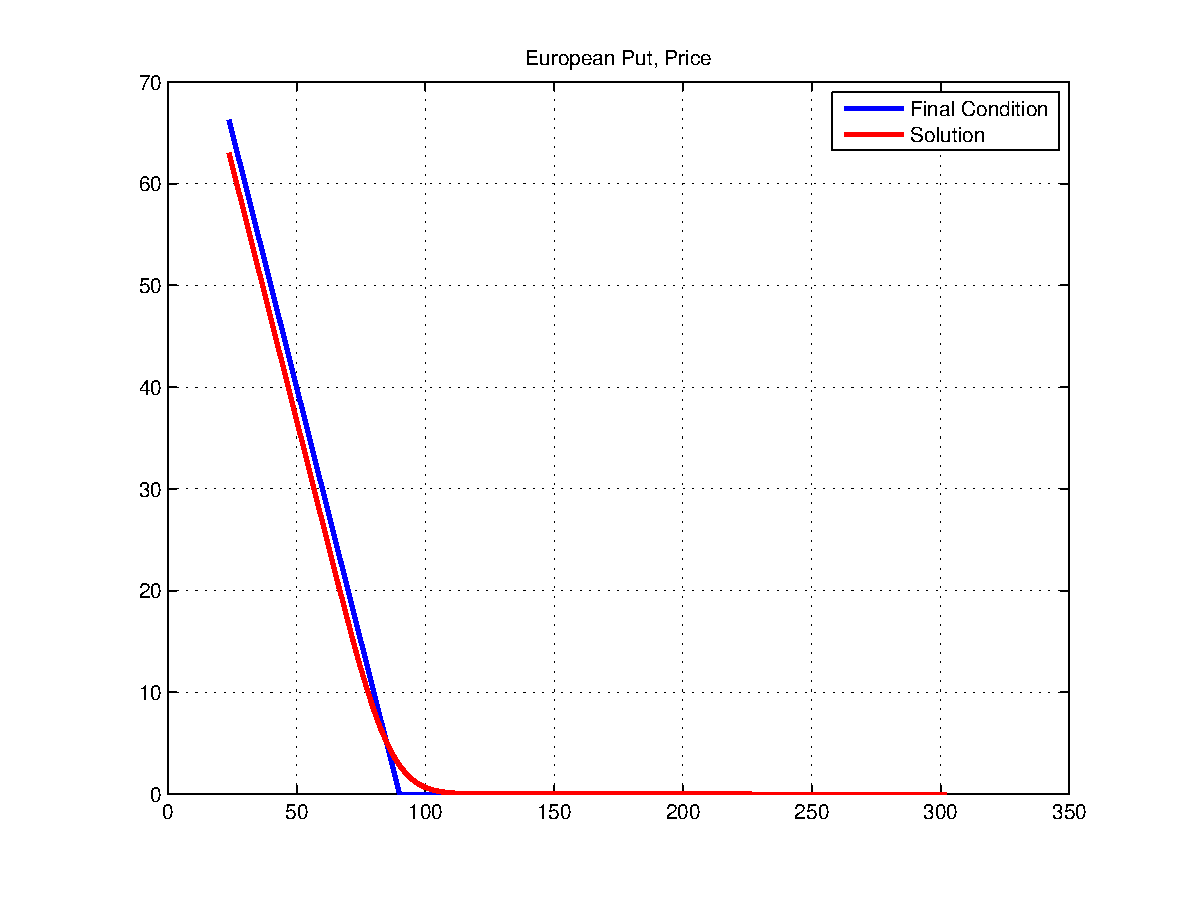
\includegraphics[width=10cm]{img/test1-put1dprice.eps}
\caption{\emph{Put} europea, con trasformazione \emph{price}}
\label{fig:test1-put1d-price}
\end{center}
\end{figure}
\begin{figure}[htp!]
\begin{center}
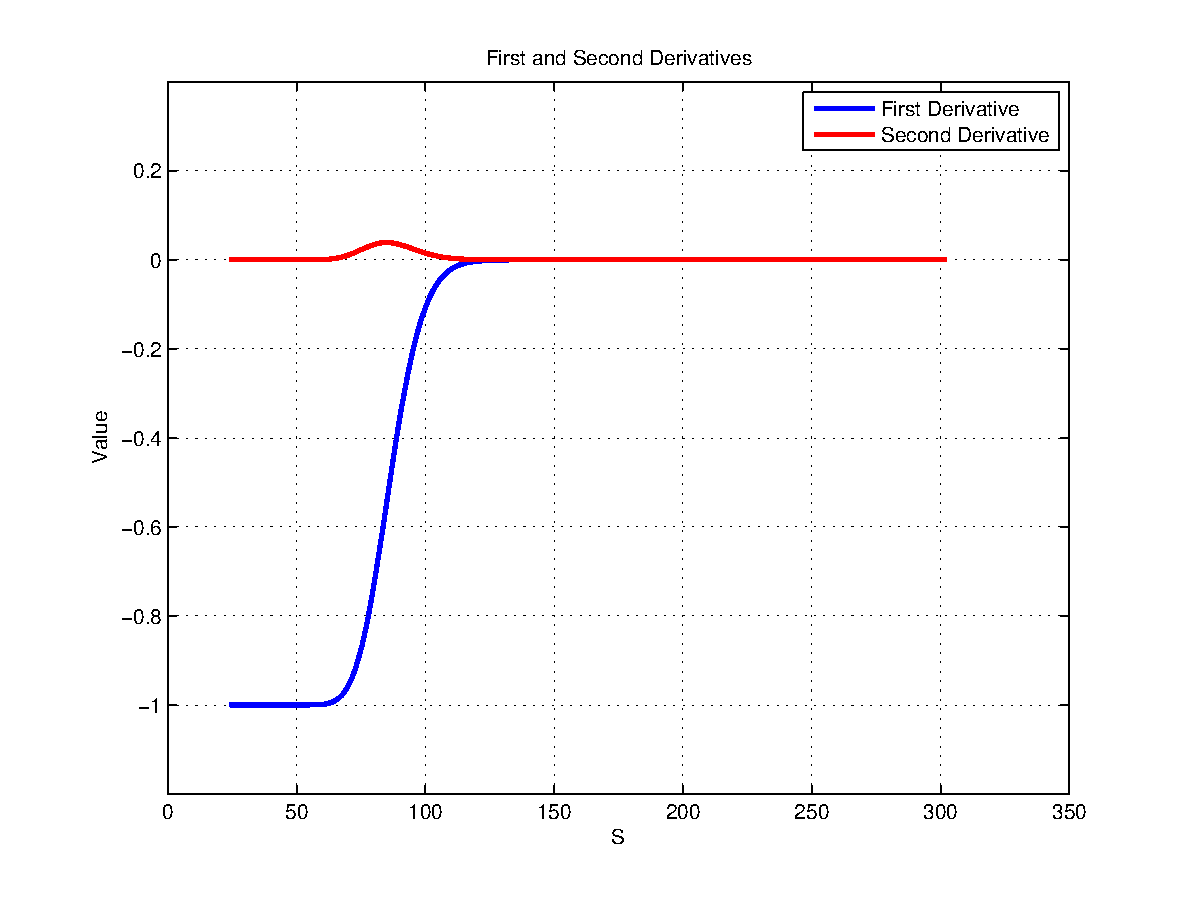
\includegraphics[width=10cm]{img/test1-derivatives.eps}
\caption{Derivata prima e seconda della \emph{put} europea, con trasformazione \emph{price}}
\label{fig:test1-derivative}
\end{center}
\end{figure}
\begin{figure}[htp!]
\begin{center}
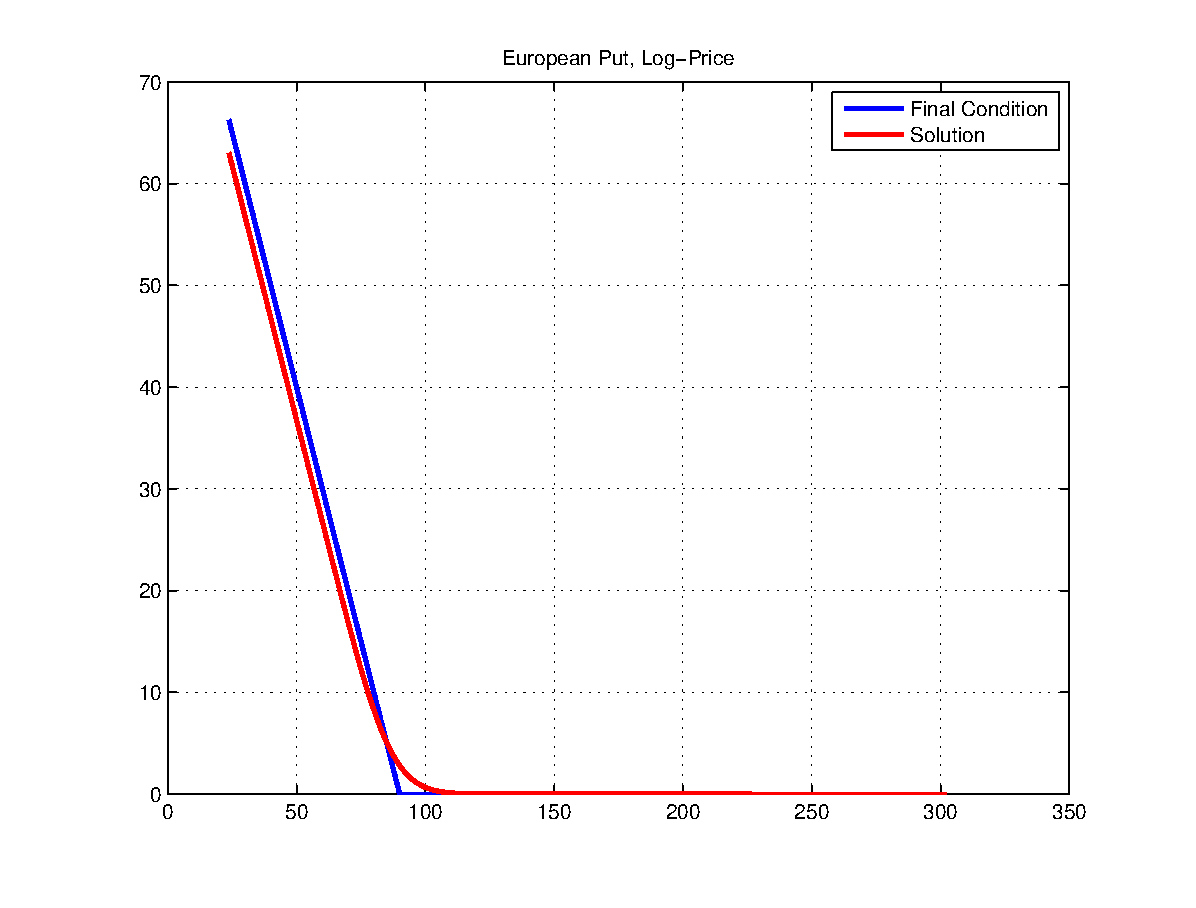
\includegraphics[width=10cm]{img/test1-put1dlogprice.eps}
\caption{\emph{Put} europea, con trasformazione \emph{log-price}}
\label{fig:test1-put1d-logprice}
\end{center}
\end{figure}
\begin{figure}[htp!]
\begin{center}
\makebox[\textwidth][c]{
\includegraphics[width=15cm]{img/test1-call2dpriceFinalC.eps}
}
\caption{\emph{Call} europea, con trasformazione \emph{price}, condizione finale}
\label{fig:test1-call1d-fc}
\end{center}
\end{figure}
\begin{figure}[htp!]
\begin{center}
\makebox[\textwidth][c]{
\includegraphics[width=15cm]{img/test1-call2dpriceSolution.eps}
}
\caption{\emph{Call} europea, con trasformazione \emph{price}, soluzione}
\label{fig:test1-call1d-sol}
\end{center}
\end{figure}
Come possiamo notare i tempi di calcolo sono davvero rapidissimi in tutti i casi. I prezzi dell'opzione monodimensionale sono identici per entrambe le trasformazioni, mentre per il 2d c'\`e una differenza apprezzabile, e aumentando il numero di elementi nella \emph{mesh} questa differenza scompare.
Nelle figure \ref{fig:test1-put1d-price}, \ref{fig:test1-put1d-logprice}, \ref{fig:test1-call1d-fc} e \ref{fig:test1-call1d-sol} sono riportati, a titolo di esempio i grafici della soluzione e della condizione finale. In figura \ref{fig:test1-derivative} abbiamo plottato la derivata prima e seconda della put europea calcolata tramite la trasformazione \emph{price}. Come possiamo vedere, queste due funzioni sono molto lisce e prive di passaggi bruschi.\\Oltre a questi semplici calcoli, abbiamo deciso di testare la convergenza del prezzo al variare della griglia, ottenendo i risultati mostrati nelle tabelle \ref{step1-2} e \ref{step1-3}. Notiamo quindi che in 1d entrambe le trasformazioni, anche con una griglia lasca e pochissimi istanti temporali, danno un risultato molto vicino al prezzo corretto, e poi convergono velocemente al prezzo esatto 9.66. In due dimensioni vediamo invece come il nostro \emph{solver} abbia bisogno di parecchi step temporali e una griglia molto fitta per dare il risultato corretto.

\begin{table}[htp!]
\begin{adjustbox}{center}
\begin{tabular}{| l | l | l | l | l | l |}
\hline
Griglia/Timesptes& 256/25 & 512/50 & 1024/100 & 2048/250 & 4196/500 \\ \hline
\emph{price} & 9.64979\officialeuro & 9.65598\officialeuro & 9.66063\officialeuro & 9.66336\officialeuro & 9.66431\officialeuro \\ \hline
\emph{log-price} & 9.64951\officialeuro & 9.65587\officialeuro & 9.66060\officialeuro & 9.66339\officialeuro & 9.66431\officialeuro \\ \hline
\end{tabular}
\end{adjustbox}
\caption{Test di convergenza per una Call 1d.}
\label{step1-2}
\end{table}

\begin{table}[htp!]
\begin{adjustbox}{center}
\begin{tabular}{| l | l | l | l | l | l |}
\hline
Griglia/Timesptes& 256/25 & 1024/50 & 4096/100 & 16384/250 & 65536/500 \\ \hline
\emph{price} & 5.13714\officialeuro & 2.88788\officialeuro & 2.63722\officialeuro & 2.54018\officialeuro & 2.49968\officialeuro \\ \hline
\emph{log-price} & 3.42608\officialeuro & 2.79298\officialeuro & 2.54516\officialeuro & 2.51124\officialeuro & 2.49826\officialeuro \\ \hline
\end{tabular}
\end{adjustbox}
\caption{Test di convergenza per una \emph{put} 2d.}
\label{step1-3}
\end{table}
\newpage
\section{\textsf{test-2}}
In questo secondo programma di esempio calcoliamo i prezzi di opzioni i cui sottostanti evolvono con modelli di L\'evy. In particolare, a titolo di esempio abbiamo prezzato delle \emph{call} europee in 1d con un modello di Kou, il cui grafico \`e riportato in figura \ref{fig:test2-call1d-kou}, e in 2d con dei modelli di Merton. I risultati ottenuti sono riportati nella tabella \ref{step2-1}.\\\\
\begin{table}[htp!]
\begin{center}
\begin{tabular}{| l | l | l | l | l | l |}
\hline
Dimensione & Trasformazione & Griglia & Timesteps & Prezzo & Tempo \\ \hline
1 & \emph{price} & 1024 & 100 & 12.4258\officialeuro & 17.3725s \\ \hline
1 & \emph{log-price} & 1024 & 100 & 12.427\officialeuro & 14.3955ss \\ \hline
2 & \emph{price} & 4096 & 100 & 23.9055\officialeuro & 14.6684s \\ \hline
2 & \emph{log-price} & 4096 & 100 & 24.0966\officialeuro & 305.049s \\ \hline
\end{tabular}
\end{center}
\caption{Prezzi di una \emph{call} 1d e 2d.}
\label{step2-1}
\end{table}
\begin{figure}[htp!]
\begin{center}
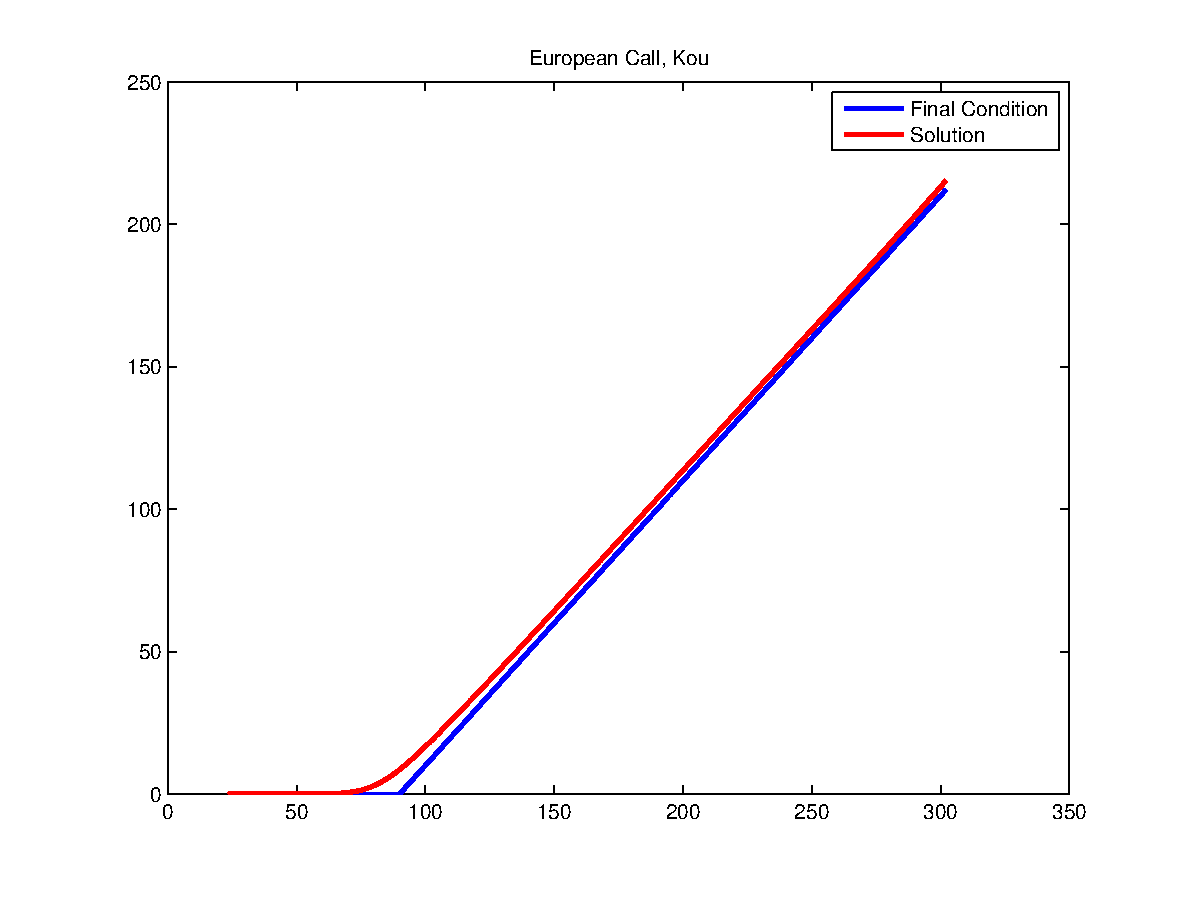
\includegraphics[width=12cm]{img/test2-call1dkou.eps}
\caption{\emph{Call} europea, con modello di Kou}
\label{fig:test2-call1d-kou}
\end{center}
\end{figure}
La prima considerazione da effettuare riguarda i tempi di calcolo: rispetto al semplice modello di \emph{Black\&Scholes}, osserviamo che i tempi impiegati per individuare il prezzo dell'opzioni sono molto maggiori. Nonostante qui le griglie siano pi\`u piccole, i tempi di calcolo per la soluzione della PIDE sono pi\`u grandi rispetto a quelli della PDE di almeno un ordine di grandezza.\\La seconda osservazione riguarda invece il confronto fra le due trasformazioni: notiamo infatti che in 1d, la trasformazione \emph{log-price} \`e pi\`u veloce rispetto alla trasformazione \emph{price}. Ci\`o \`e dovuto al fatto che l'implementazione della parte integrale in \emph{log-price}, pur essendo pi\`u pesante rispetto all'altra, poich\'e occorre ogni volta calcolare dei valori della soluzione in punti non noti a priori della griglia, permette un'immediata parallelizzazione, mentre la trasformazione \emph{price}, in teoria pi\`u rapida, non \`e facilmente parallelizzabile. Quindi, la risoluzione del problema con la trasformazione \emph{price} \`e s\`i pi\`u veloce da un punto di vista algoritmico, ma in questo particolare caso, con a disposizione 4 processori, la trasformazione \emph{log-price} ha prestazioni di poco migliori.\\In due dimensioni, invece, le prestazioni della trasformazione \emph{log-price} non reggono il paragone rispetto a \emph{price}. Questo è dovuto al fatto che in due dimensioni la ricerca delle celle in cui si trovano i punti in cui deve essere valutata la soluzione diventa molto più onerosa, trattandosi di una griglia bidimensionale.\\\\
\begin{figure}[htp!]
\begin{center}
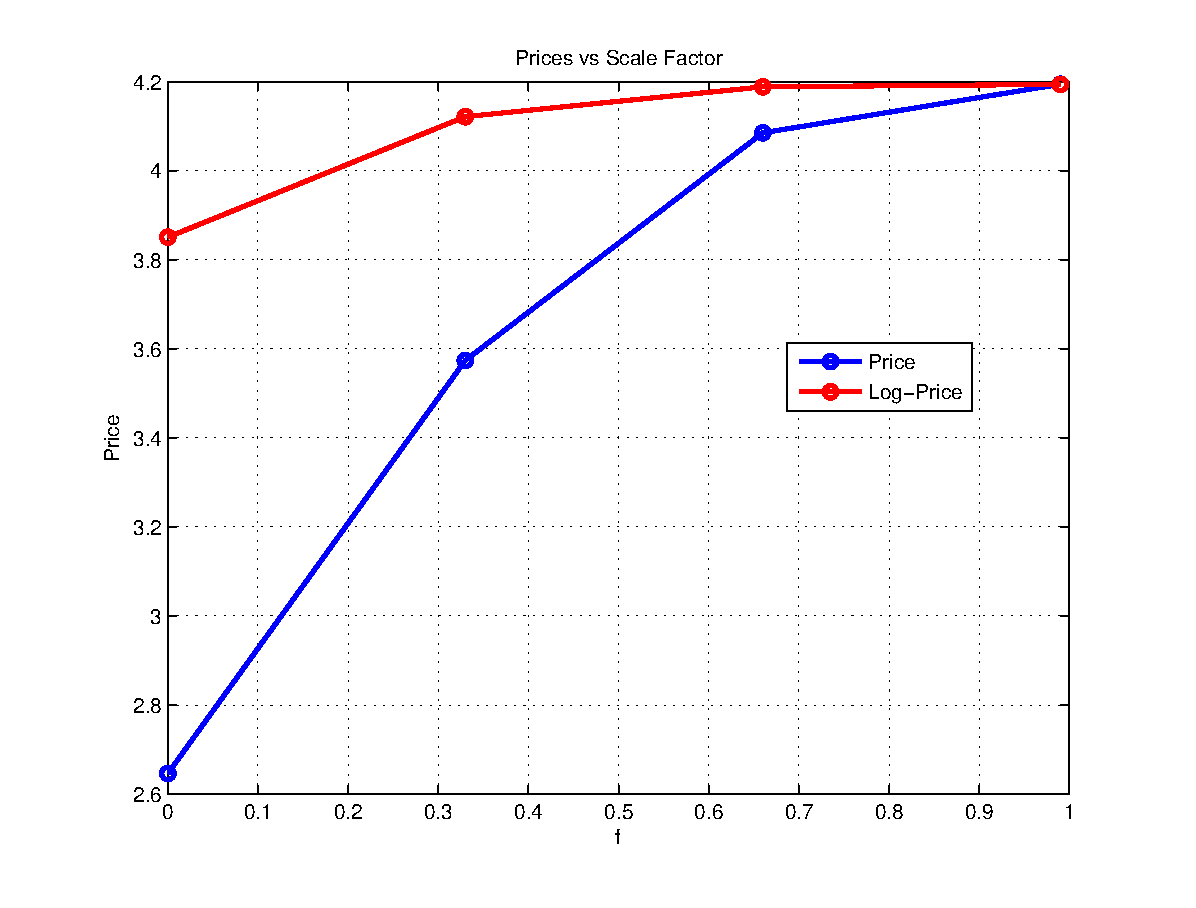
\includegraphics[width=12cm]{img/test2-scalefactor.eps}
\caption{Prezzi di una \emph{put} con modello di Kou, al variare di $f$.}
\label{fig:test2-scalefactor}
\end{center}
\end{figure}
Un altro test effettuato in questo programma \`e il calcolo del prezzo al variare del fattori di scala $f$, introdotto in \eqref{cut}. Testando infatti il comportamento della libreria, ci siamo resi conto che i prezzi delle opzioni erano leggermente inferiori ai prezzi target, specialmente nella trasformazione \emph{price}. Nella figura \ref{fig:test2-scalefactor} possiamo osservare l'andamento dei prezzi nelle due trasformazioni all'aumentare del fattore di scala. Come accennato in precedenza, un fattore di scala piccolo determina un grosso errore nella valutazione di questo tipo di opzioni nella trasformazione \emph{price}. Ci\`o \`e dovuto al fatto che la griglia su cui risolviamo la PDE in questa trasformazione coincide con la griglia su cui calcoliamo l'integrale: se il troncamento \`e troppo elevato rischiamo di perdere dei contributi importanti della parte integrale. La trasformazione \emph{log-price} invece risente meno di questo problema poich\'e grazie ai nodi di quadratura di Hermite e di Laguerre il dominio di integrazione non \`e troncato, ma coincide con tutto l'asse reale, e infatti con questa trasformazione l'errore con $f$ piccolo \`e contenuto e all'aumentare di $f$ converge velocemente al valore esatto.\\\\Infine, abbiamo studiato come varia il prezzo della trasformazione \emph{log-price} al variare dei nodi di quadratura: il programma permette infatti di adattare la quadratura numerica in modo da scendere al di sotto di errore target. Nella tabella \ref{step2-2}, mostriamo la variazione di prezzo all'aumentare dei nodi di quadratura.\\
\begin{table}[htp!]
\begin{adjustbox}{center}
\begin{tabular}{| l | l | l | l | l | l | l |}
\hline
$\#$ di nodi & 4 & 8 & 16 & 32 & 64 & 128 \\ \hline
Prezzi & 12.095\officialeuro & 12.4534\officialeuro & 12.4279\officialeuro & 12.427\officialeuro & 12.4264\officialeuro & 12.4264\officialeuro \\ \hline
Tempi & 4.08526s	&	6.47795s	&	9.47712s	&	14.4233s	&	20.2579s & 28.1988s \\ \hline
\end{tabular}
\end{adjustbox}
\caption{Prezzi e tempi di calcolo del prezzo di \emph{call} 1d al variare dei nodi di quadratura.}
\label{step2-2}
\end{table}
Come possiamo notare, la differenza di prezzo all'aumentare dei nodi di quadratura \`e davvero irrisoria. Ci\`o \`e probabilmente dovuto al fatto che nonostante l'errore sul vettore $J$ possa essere grande, esso viene moltiplicato per la matrice di massa, che generalmente ha numeri molto piccoli. Per questo un errore pur grande su $J$ si manifesta in misura molto attenuata nel prezzo finale. Inoltre, all'aumentare dei nodi di quadratura il tempo di calcolo aumenta considerevolmente. Per questo motivo abbiamo deciso di settare come numero massimo di nodi 32 (ovviamente modificabile con un apposito metodo), in quanto ci sembra l'equilibrio giusto fra precisione e velocit\`a di calcolo.
\section{\textsf{test-3}}
In questo programma abbiamo mostrato come risolvere il problema con l'ostacolo, ovvero come calcolare il prezzo di opzioni americane. Inizialmente, abbiamo calcolato i prezzi di opzioni con modelli di \emph{Black\&Scholes} in una e due dimensioni, ottenendo i risultati in \ref{test3-1}.
\begin{table}[htb!]
\begin{center}
\begin{tabular}{| l | l | l | l | l | l |}
\hline
Dimensione & Trasformazione & Griglia & Timesteps & Prezzo & Tempo \\ \hline
1 & \emph{price} & 1024 & 100 & 1.54933\officialeuro & 0.885832s \\ \hline
1 & \emph{log-price} & 1024 & 100 & 1.54931\officialeuro & 1.08148s \\ \hline
2 & \emph{price} & 16384 & 100 & 4.43963\officialeuro & 1.2148s \\ \hline
2 & \emph{log-price} & 16384 & 100 & 4.41147\officialeuro & 0.990322s \\ \hline
\end{tabular}
\end{center}
\caption{Prezzi di \emph{put} americane 1d e 2d, \emph{Black\&Scholes}.}
\label{test3-1}
\end{table}
Il nostro \emph{solver}, che \`e in grado di lavorare anche in parallelo, sembra comportarsi molto bene, sia per quanto riguarda la velocit\`a di calcolo che la precisione raggiunta: la tolleranza per bloccare il \emph{solver} iterativo \`e infatti impostata a $10^{-10}$ e le iterazioni massime sono 1000. Qualora il \emph{solver} non dovesse convergere alla tolleranza in 1000 iterazioni, il programma stampa un \emph{warning}, avvisando l'utente di aver raggiunto il numero massimo di iterazioni e riportando l'errore attuale. Calcolando i prezzi precedenti con una griglia pi\`u fitta il \emph{solver} stampa il \emph{warning}, ma arriva comunque a un errore minore di $10^{-9}$, un valore decisamente accettabile.\\\\Oltre al modello di \emph{Black\&Scholes}, abbiamo anche utilizzato un modello di Kou, per calcolare il prezzo di un'opzione americana monodimensionale. Con una griglia di 1024 celle e 100 iterazioni temporali otteniamo i seguenti prezzi riportati in \ref{test3-2}.
\begin{table}[htb!]
\begin{center}
\begin{tabular}{| l | l | l |}
\hline
Trasformazione & Prezzo & Tempo \\ \hline
\emph{price} & 4.42944\officialeuro & 22.9670s \\ \hline
\emph{log-price} & 4.4122\officialeuro & 13.4689s \\ \hline
\end{tabular}
\end{center}
\caption{Prezzi di una \emph{put} americana, Kou.}
\label{test3-2}
\end{table}
Come possiamo notare i prezzi sono simili per entrambe le trasformazioni, mentre i tempi di calcolo rispecchiano il comportamento delle PIDE 1d mostrato in \ref{step2-1}. In figura \ref{fig:test2-putamkou} possiamo apprezzare come la soluzione stia sempre sopra alla condizione finale, cosa che per esempio non avviene in figura \ref{fig:test1-put1d-price}, che descrive il comportamento di una \emph{put} europea. Nel secondo grafico invece della figura \ref{fig:test2-putamkou} abbiamo plottato la derivata prima e la derivata seconda della soluzione: a differenza di quanto accade nella figura \ref{fig:test1-derivative}, qui possiamo vedere come esse siano molto ``lisce'' fino al punto di contatto con l'ostacolo, dove notiamo un cambio un po' brusco di inclinazione. Ci\`o \`e dovuto al fatto che da quel punto in poi, nonostante la soluzione tenda a scendere sotto l'ostacolo, il \emph{solver} impone che la soluzione sia pari al \emph{payoff}.
\begin{figure}[htp!]
\begin{center}
\includegraphics[width=\textwidth]{img/test2-putamkou.eps}
\caption{\emph{Put} americana, con trasformazione \emph{price}.}
\label{fig:test2-putamkou}
\end{center}
\end{figure}
\newpage
\section{\textsf{test-4}}
Il \textsf{test-4} permette di confrontare le prestazioni e in particolare lo \emph{speed-up} del calcolo dell'integrale in \emph{log-price} sfruttando il calcolo parallelo. Il programma permette di confrontare la velocit\`a del calcolo effettuato con uno e con il numero di processori disponibili sul computer. Oltre a questo, per analizzare nel dettaglio il comportamento del nostro programma, lo abbiamo anche testato con pi\`u \emph{threads} rispetto ai processori disponibili. Nelle tabelle \ref{speedtest1d} e \ref{speedtest2d} sono riportati i risultati che riassumono l'andamento dell'accelerazione permessa dal \emph{multi-threading}.
\begin{table}[htp!]
\begin{center}
\begin{tabular}{| l | l | l | l |}
\hline
Griglia & Prezzo & Tempo & \emph{speed-up} \\ \hline
\multicolumn{4}{| l |} {1 \emph{thread}:} \\ \hline
256	& 12.4289\officialeuro		& 7.69022s		& \\ \hline
512	& 12.4264\officialeuro		& 18.4018s		& \\ \hline
1024	& 12.4264\officialeuro		& 48.7283s		& \\ \hline
2048	& 12.4264\officialeuro		& 145.728s		&  \\ \hline
\multicolumn{4}{| l |} {2 \emph{threads}:} \\ \hline
256	& 12.4289\officialeuro		& 4.84786s		& 1.5863x\\ \hline
512	& 12.4264\officialeuro		& 11.6194s		& 1.5837x\\ \hline
1024	& 12.4264\officialeuro		& 28.5346s		& 1.7077x\\ \hline
2048	& 12.4264\officialeuro		& 82.5946s		& 1.7644x\\ \hline
\multicolumn{4}{| l |} {4 \emph{threads}:} \\ \hline
256	& 12.4289\officialeuro		& 3.63051s		& 2.11822x \\ \hline
512	& 12.4264\officialeuro		& 7.72159s		& 2.38316x \\ \hline
1024	& 12.4264\officialeuro		& 18.1312s		& 2.68754x \\ \hline
2048	& 12.4264	\officialeuro	& 51.4363s		& 2.83317x \\ \hline
\multicolumn{4}{| l |} {8 \emph{threads}:} \\ \hline
256	& 12.4289\officialeuro		& 4.19548s		& 1.83298x \\ \hline
512	& 12.4264\officialeuro		& 9.01837s		& 2.04048x \\ \hline
1024	& 12.4264\officialeuro		& 21.2442s		& 2.29372x \\ \hline
2048	& 12.4264\officialeuro		& 57.4038s		& 2.53865x \\ \hline
\end{tabular}
\end{center}
\caption{\emph{Speed test} 1d}
\label{speedtest1d}
\end{table}

\begin{table}[htp!]
\begin{center}
\begin{tabular}{| l | l | l | l |}
\hline
Griglia & Prezzo & Tempo & \emph{speed-up} \\ \hline
\multicolumn{4}{| l |} {1 \emph{thread}:} \\ \hline
256		& 19.3305\officialeuro		& 19.6544	s	& \\ \hline
1024		& 17.6665\officialeuro		& 112.993s		& \\ \hline
4096		& 17.3574\officialeuro		& 1029.37s		& \\ \hline
16384	& 17.2674\officialeuro		& 12921s		& \\ \hline
\multicolumn{4}{| l |} {2 \emph{threads}:} \\ \hline
256		& 19.3305\officialeuro		& 11.1107s		& 1.7690x \\ \hline
1024		& 17.6665	\officialeuro		& 60.4006s		& 1.8707x \\ \hline
4096		& 17.3595\officialeuro		& 560.834s		& 1.8354x \\ \hline
16384	& 17.2674\officialeuro		& 6773.54s		& 1.9076x \\ \hline
\multicolumn{4}{| l |} {4 \emph{threads}:} \\ \hline
256		& 19.3305\officialeuro		& 7.2931s			& 2.6949x \\ \hline
1024		& 17.6665\officialeuro		& 39.4015s		& 2.8677x \\ \hline
4096		& 17.3595\officialeuro		& 348.897s		& 2.9504x \\ \hline
16384	& 17.2674\officialeuro		& 4229.25s		& 3.0552x \\ \hline
\multicolumn{4}{| l |} {8 \emph{threads}:} \\ \hline
256		& 19.3305\officialeuro		& 10.4722s		& 1.87681x \\ \hline
1024		& 17.6665\officialeuro		& 50.4595s		& 2.23928x \\ \hline
4096		& 17.3595\officialeuro		& 369.883s		& 2.78296x \\ \hline
16384	& 17.2674\officialeuro		& 42204s			& 3.06159x \\ \hline
\end{tabular}
\end{center}
\caption{\emph{Speed test} 2d}
\label{speedtest2d}
\end{table}
Volendo ora applicare la Legge di Amdahl, possiamo calcolare lo \emph{speed-up} teorico massimo possibile e confrontarlo con quello da noi ottenuto. In particolare, la Legge di Amdhal afferma che l'accelerazione massima possibile sfruttando il calcolo parallelo \`e data dalla seguente equazione: $$A_{max}=\frac{1}{(1-P)+\frac{P}{S}},$$in cui $A_{max}$ indica l'accelerazione massima, $S$ il numero di \emph{threads} e $P$ è la frazione di tempo che la parte parallelizzata impiega se eseguita in seriale. Nel nostro caso, come possiamo osservare in figura \ref{fig:callgraph}, il calcolo dell'integrale effettuato tramite la funzione \textsf{get\_one\_J()} impiega il $99.59\%$, quindi dobbiamo porre $P=0.9959$. L'accelerazione massima teorica \`e quindi $1.9918$x per 2 \emph{cores} e $3.9514$x per 4 \emph{cores}.
\begin{figure}[htp!]
\begin{center}
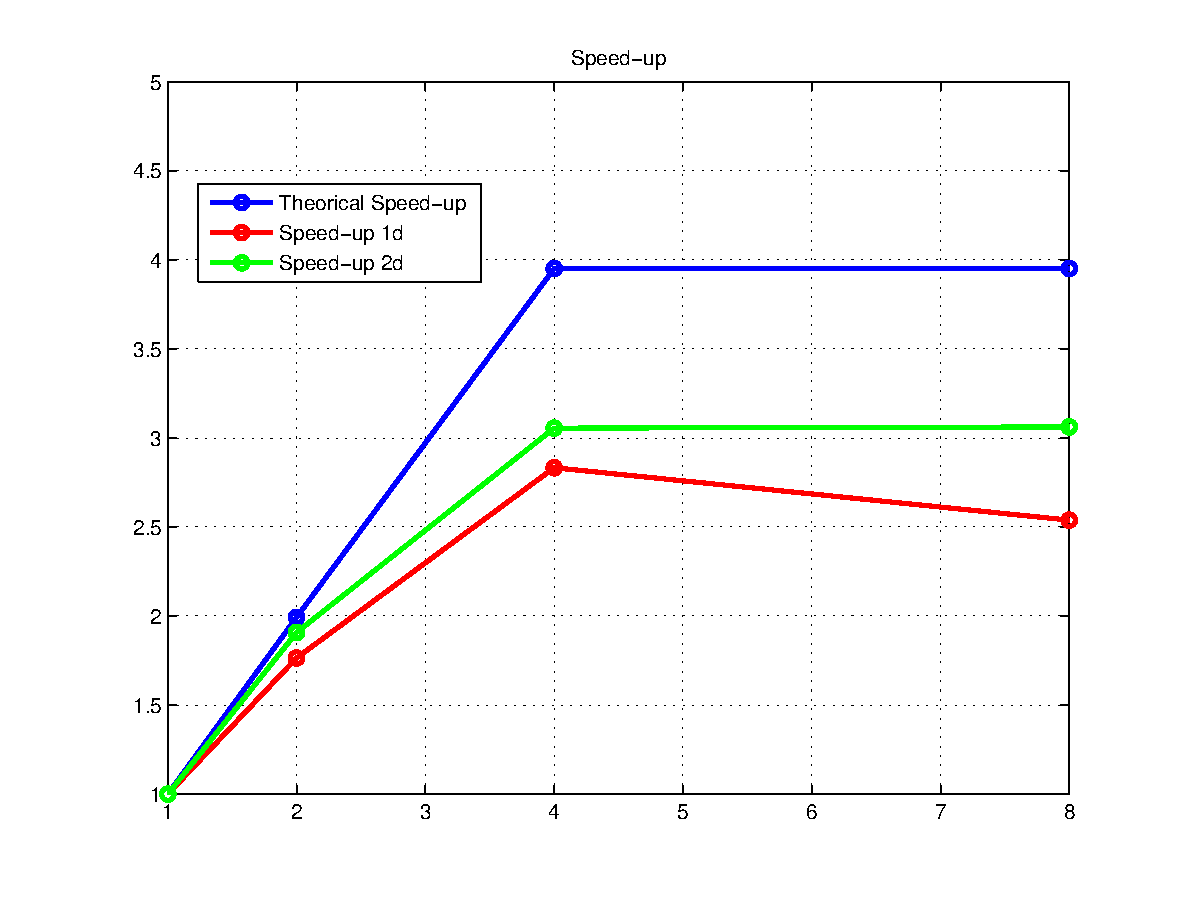
\includegraphics[width=12cm]{img/test4-speedup.eps}
\caption{Plot degli \emph{speed-up} su un processore quad-core.}
\label{test4:speedup}
\end{center}
\end{figure}
Come possiamo osservare in figura \ref{test4:speedup}, non riusciamo a raggiungere lo \emph{speed-up} teorico prossimo ai 4x stimato dalla legge di Amdahl, probabilmente perch\'e il computer su cui abbiamo testato il programma non \`e molto adatto al calcolo parallelo: le prestazioni con due \emph{threads} infatti sono vicine al limite teorico 1.99x, mentre 4 \emph{threads} su 4 \emph{cores} non riescono a sfruttare il 100\% delle prestazioni del processore. Riteniamo che il motivo per cui questo accade \`e che alcune risorse vengano assorbite dal sistema operativo e dalla gestione dei vari processi. Questa conclusione a cui siamo giunti \`e avvalorata dal fatto che anche con 8 \emph{threads} le prestazioni sono uguali o addirittura peggiorano nell'1d, poich\'e proprio il computer fatica a gestire molti \emph{threads} computazionalmente onerosi.\\Infine, non possiamo non notare che i tempi di calcolo sfruttando tutti e quattro i \emph{cores} sono decisamente migliori rispetto al calcolo seriale, permettendo cos\`i alla trasformazione \emph{log-price} di competere e addirittura superare da un punto di vista di velocit\`a di calcolo la trasformazione \emph{price} nell'1d.
\newpage
\section{\textsf{test-5}}
In quest'ultimo test abbiamo valutato le prestazioni della nostra libreria attivando il flag del \emph{mesh refinement}. In particolare, l'abbiamo provato con opzioni monodimensionali in entrambe le trasformazioni, e nel caso bidimensionale per il \emph{log-price}. I risultati ottenuti nel caso 1d sono riportati nella tabella \ref{test5-1}.
\begin{table}[htb!]
\begin{adjustbox}{center}
\begin{tabular}{| l | l | l | l | l | l | l |}
\hline
Trasformazione & Celle di partenza & Celle di arrivo & Timesteps & Prezzo & Tempo \\ \hline
\emph{price} & 256 & 520 & 100 & 12.4267\officialeuro & 2.74439s \\ \hline
\emph{log-price} & 256 & 520 & 100 & 12.4281\officialeuro & 4.23711s \\ \hline
\end{tabular}
\end{adjustbox}
\caption{Prezzi di una \emph{call} 1d, Kou, con parametri 0.2 di \emph{refinement} e 0.03 di \emph{coarsening}.}
\label{test5-1}
\end{table}
Questi risultati sono stati ottenuti con il medesimo modello utilizzato per il caso monodimensionale di \ref{step2-1}, e come possiamo notare, non solo i prezzi ottenuti sono praticamente gli stessi, ma sono calcolati molto pi\`u velocemente, in particolare per la trasformazione \emph{price}.\\Oltre alle opzioni europee, abbiamo testato il \emph{mesh refinement} anche sulle opzioni americane, con risultati non pienamente soddisfacenti. Come gi\`a detto infatti, i prezzi di queste opzioni viene calcolato mediante un \emph{solver} iterativo, che con l'adattivit\`a di griglia fatica a convergere. Abbiamo quindi calcolato i prezzi di una semplice opzione americana con il modello di \emph{Black\&Scholes} al variare delle iterazioni massime del \emph{solver}, ottenendo i risultati illustrati nelle tabelle \ref{test5-2} e \ref{test5-3}. I prezzi target sono quelli monodimensionali riportati in \ref{test3-1}, e come possiamo vedere i prezzi faticano a convergere, anche con 1000 iterazioni massime (ovvero il parametro di default). Ipotizziamo che, a causa del riordinamento dei nodi e aggiunta di altri, la matrice diventi mal condizionata e per questo motivo il \emph{solver} faccia fatica a convergere.
\begin{table}[htb!]
\begin{center}
\begin{tabular}{| l | l | l | l |}
\hline
Maxiter & 100 & 1000 & 10000 \\ \hline
Prezzo & 1.09713\officialeuro & 1.46016\officialeuro	& 1.54845\officialeuro \\ \hline
Tempo & 0.54812s	& 3.79223s & 18.0422s\\ \hline
\end{tabular}
\end{center}
\caption{Prezzi di una \emph{put} americana in \emph{price}, con parametri 0.2 di \emph{refinement} e 0.03 di \emph{coarsening}.}
\label{test5-2}
\end{table}
\begin{table}[htb!]
\begin{center}
\begin{tabular}{| l | l | l | l |}
\hline
Maxiter & 100 & 1000 & 10000\\ \hline
Prezzo & 1.26063\officialeuro &	1.50763\officialeuro & 1.52639\officialeuro \\ \hline
Tempo & 0.851332s	 & 5.55052es & 17.7176s\\ \hline
\end{tabular}
\end{center}
\caption{Prezzi di una \emph{put} americana in \emph{log-price}, con parametri 0.2 di \emph{refinement} e 0.03 di \emph{coarsening}.}
\label{test5-3}
\end{table}

Ci siamo infine concentrati sull'adattivit\`a di griglia nelle opzioni bidimensionali, con la trasformazione \emph{log-price} (ricordiamo infatti che poich\'e il \emph{price} richiede una griglia strutturata, non \`e corretto fare \emph{mesh adapting}). Abbiamo quindi testato il comportamento di una \emph{call} 2d al variare dei coefficienti di adattivit\`a, i cui sottostanti evolvono secondo modelli di Merton, ottenendo i risultati riportati in \ref{test5-4}.
\begin{table}[htb!]
\begin{adjustbox}{center}
\begin{tabular}{| l | l | l | l | l | l | l |}
\hline
Ref/Coar & g.d.l di partenza & g.d.l di arrivo & Timesteps & Prezzo & Tempo \\ \hline
0.03/0.15 & 4225 & 4780 & 100 & 24.1053\officialeuro & 357.969s \\ \hline
0/0.1 & 4225 & 3526 & 100 & 24.097\officialeuro & 275.006s \\ \hline
\end{tabular}
\end{adjustbox}
\caption{Prezzi di una \emph{call} 2d, Merton.}
\label{test5-4}
\end{table}
Questi valori sono da confrontare con quelli riportati nella tabella \ref{step2-1}. Come possiamo notare, qui i prezzi convergono al valore giusto, con tempi di calcolo coerenti rispetto alle prestazioni del caso senza raffinamento di griglia: nel primo caso infatti, all'aumentare dei nodi, il programma impiega pi\`u tempo a girare, rispetto a quanto indicato in \ref{step2-1}, mentre nel secondo caso, i nodi della griglia diminuiscono, permettendo all'algoritmo di calcolare il prezzo in modo pi\`u rapido. L'accelerazione nel secondo caso tuttavia non \`e molto evidente, ci\`o \`e dovuto sia al fatto che i nodi non diminuiscono cos\`i tanto e poi con il \emph{mesh refinement}, il programma ogni 20 iterazioni temporali deve ricostruire il sistema, impiegando un tempo non trascurabile.\\Di seguito sono riportate le \emph{mesh} generate nei due casi: nel set con parametri 0.03/0.15 possiamo vedere come la griglia diventi pi\`u lasca nella parte in cui la soluzione \`e nulla e dove la soluzione cresce in modo costante, mentre si infittisce dove la soluzione si alza e vicino ai bordi, dove c'\`e una condizione al contorno $\mathcal{C}^0$. Nel set di griglie con parametri 0/0.1 notiamo invece come la soluzione diventi pi\`u lasca nella zona in cui la soluzione vale 0.
\begin{figure}[htp!]
\begin{center}
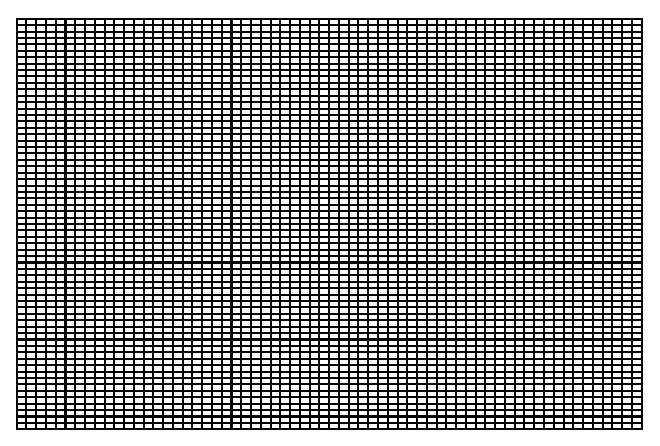
\includegraphics[width=10cm]{img/meshes/Price1.eps}
\caption{Griglia iniziale.}
\label{fig:test5-price1}
\end{center}
\end{figure}
\begin{figure}[htp!]
\begin{center}
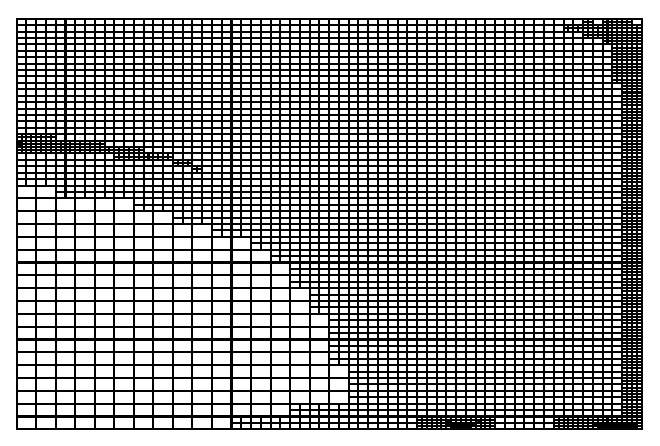
\includegraphics[width=10cm]{img/meshes/Price2.eps}
\caption{Griglia dopo 2 step di raffinamento, con parametri 0.03 di \emph{refinement} e 0.15 di \emph{coarsening}.}
\label{fig:test5-price2}
\end{center}
\end{figure}
\begin{figure}[htp!]
\begin{center}
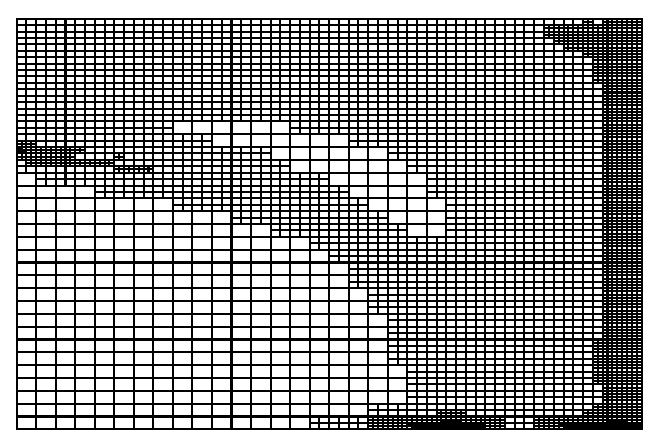
\includegraphics[width=10cm]{img/meshes/Price3.eps}
\caption{Griglia dopo 4 step di raffinamento, con parametri 0.03 di \emph{refinement} e 0.15 di \emph{coarsening}.}
\label{fig:test5-price3}
\end{center}
\end{figure}

\begin{figure}[htp!]
\begin{center}
\makebox[\textwidth][c]{
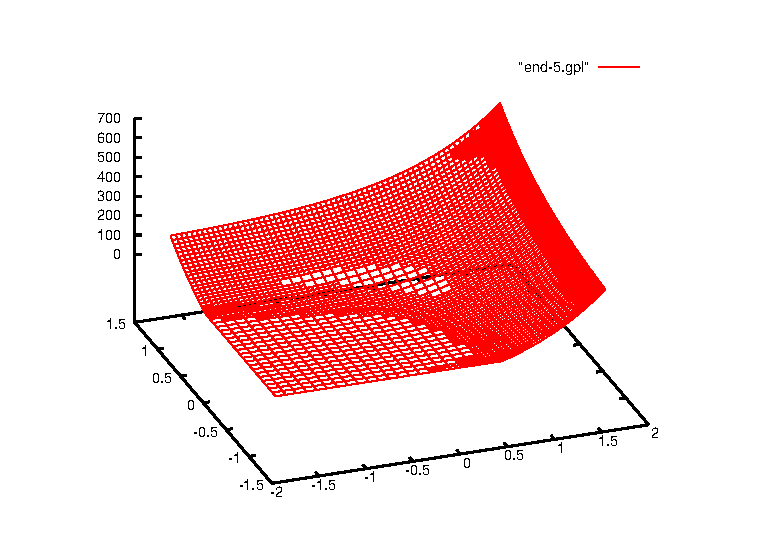
\includegraphics[width=15cm]{img/test5-1.eps}
}
\caption{Valore della soluzione di una \emph{call} 2d \emph{log-price}, con parametri 0.03 di \emph{refinement} e 0.15 di \emph{coarsening}.}
\label{fig:test5-1}
\end{center}
\end{figure}

\begin{figure}[htp!]
\begin{center}
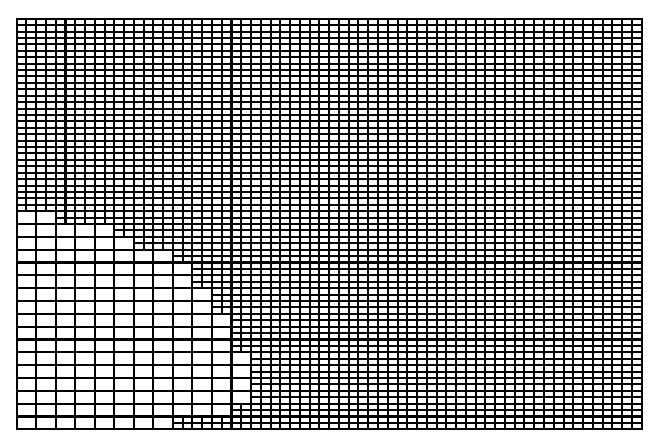
\includegraphics[width=10cm]{img/meshes/LogPrice2.eps}
\caption{Griglia dopo 2 step di raffinamento, con parametri 0 di \emph{refinement} e 0.1 di \emph{coarsening}.}
\label{fig:test5-logprice2}
\end{center}
\end{figure}
\begin{figure}[htp!]
\begin{center}
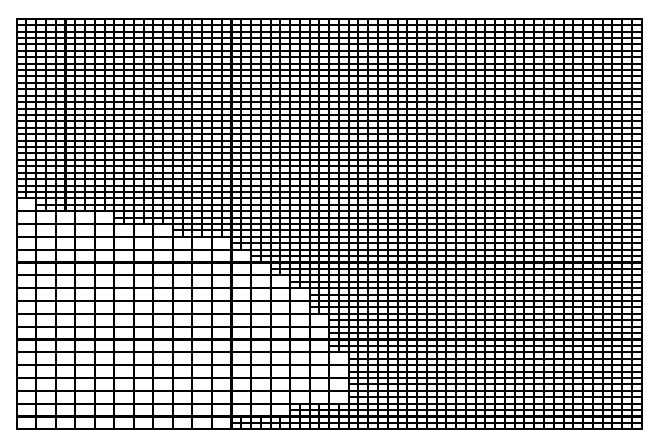
\includegraphics[width=10cm]{img/meshes/LogPrice3.eps}
\caption{Griglia dopo 4 step di raffinamento, con parametri 0 di \emph{refinement} e 0.1 di \emph{coarsening}.}
\label{fig:test5-logprice3}
\end{center}
\end{figure}


\begin{figure}[htp!]
\begin{center}
\makebox[\textwidth][c]{
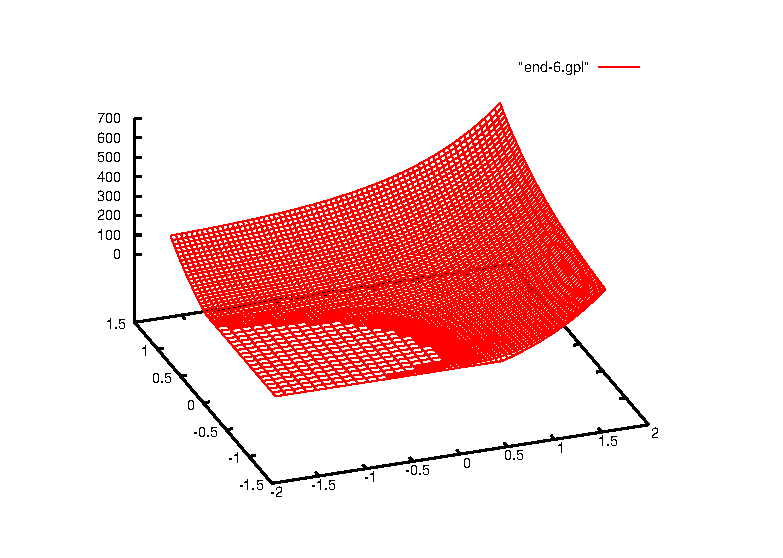
\includegraphics[width=15cm]{img/test5-2.eps}
}
\caption{Valore della soluzione di una \emph{call} 2d \emph{log-price}, con parametri 0 di \emph{refinement} e 0.1 di \emph{coarsening}.}
\label{fig:test5-2}
\end{center}
\end{figure}

\chapter{Estensioni}
Il programma che abbiamo scritto si presta molto a possibili estensioni, su molti livelli. In particolare, a partire dalle classi base \textsf{OptionBasePrice$<$dim$>$} e \textsf{OptionBaseLogPrice$<$dim$>$} \`e possibile scrivere dei \emph{solver} che prezzino tutte le opzioni barriera, ovvero opzioni caratterizzate da condizioni al bordo di \emph{Dirichlet} nulle in alcune parti o su tutto il bordo dominio, che riflettono il fatto che se il sottostante tocca tali barriere l'opzione ha valore nullo.\\\`E inoltre possibile estendere la libreria in modo che prezzi opzioni con altri modelli, per esempio ad attivit\`a infinita, caratterizzati cio\`e da misure di L\'evy non limitate (come, ad esempio, il \emph{Normal Inverse Gaussian} e il \emph{Variance Gamma}). Per fare ci\`o occorre modificare le classi integrale, in modo che calcolino il parametro $\lambda$, che per questi modelli \`e incognito e calcolare all'interno della classe opzione la diffusione che approssima i piccoli salti (che in questo caso, sono infiniti).\\Un'altra estensione possibile, ma abbastanza delicata, \`e estendere il programma al calcolo di opzioni con tre sottostanti, ovvero risolvere un PIDE 3d. Teoricamente l'equazione sarebbe formalmente la stessa, con l'aggiunta di un terzo integrale su $\mathbb{R}$. Occorrerebbe tuttavia prestare attenzione a dove integrare i vari integrali: in 2d, infatti, nella trasformazione \emph{price} abbiamo calcolato gli integrali sui lati dei quadrilateri che costituiscono la \emph{mesh}, in 3d si dovrebbe invece integrare sui lati delle facce dei parallelepipedi. Teoricamente, cos\`i come \textsf{deal.ii} offre la possibilità di lavorare sulle facce di celle bidimensionali, permette anche di lavorare su facce e spigoli nel caso tridimensionale. \\Si potrebbe provare poi a utilizzare le funzioni offerte dalla libreria \textsf{deal.ii} per la soluzione del problema con memoria distribuita. Per quanto riguarda la parte PDE si pu\`o sfruttare quanto implementato nella libreria, mentre per il calcolo dell'integrale in \emph{price} occorrerebbe spedire tutta la soluzione a tutti i processi (perch\'e il termine \`e non locale), in \emph{log-price} invece tutti i processi devono conoscere tutta la griglia, per poter valutare la funzione nei punti $y+x$ (\ref{intnonlocal}).\\\\
Proprio perché molto semplice, abbiamo creato due piccole estensioni a titolo illustrativo.
\begin{description}[leftmargin=0cm]
 \item[\bf doubling\_extension] \hfill \\ Un'estensione che cambia il modo di stimare l'errore per il \emph{mesh refinement}. Ereditando da \textsf{EuropeanOptionLogPrice}, reimplementa i metodi \textsf{solve} e \textsf{refine\_grid}, e definisce due nuovi metodi: \textsf{solve\_one\_step} e \textsf{estimate\_doubling}. Per stimare l'errore, si procede nel modo seguente. La soluzione e la griglia attuale vengono messe da parte, e si raffina ogni cella della griglia, ottenendo una griglia fine. Su questa si trasferisce la soluzione tramite interpolazione e si risolve il problema, ottenendo una nuova soluzione sulla griglia fine. Questa soluzione ottenuta sulla griglia più fine viene poi interpolata sulla griglia originale, ed in ogni cella si calcola, per ogni grado di libert\`a della cella, l'errore scarto quadratico ra soluzione sulla griglia fine e quella \emph{coarse}. L'errore nella cella è dato dalla somma degli errori dei suoi gradi di libertà. In seguito si procede a raffinare le celle con un errore pi\`u grande e deraffinare quelle con un errore pi\`u basso. 
 
 \item[\bf barrier\_extension]  \hfill \\ Questa estensione, permette di calcolare il prezzo di una opzione barriera \emph{call up\&out}. Questo tipo di opzioni sono caratterizzate da un \emph{payoff} nella forma seguente: $$C(S(t),t)=max(S_T-K,0)\mathcal{I}_{\{S_t<H, t\in[0,T]\}},$$ ovvero queste opzioni pagano il \emph{payoff} a scadenza se e solo se il sottostante non ha mai superato la barriera $H$ in $[0,T]$. Per il \emph{pricing} di queste opzioni occorre in primo luogo troncare il dominio in corrispondenza della barriera $H$ e imporre condizioni al bordo nulle sui lati della \emph{mesh} in cui \`e presente la barriera. Come possiamo notare in figura \ref{fig:barrier}, il problema ha in questo caso condizioni al contorno nulle ovunque: su due lati infatti, occorre imporre la condizione della \emph{call} (che \`e nulla), sugli altri due lati invece si impongono condizioni al bordo nulle per la presenza delle barriere.
 \begin{figure}[htp!]
\begin{center}
\makebox[\textwidth][c]{
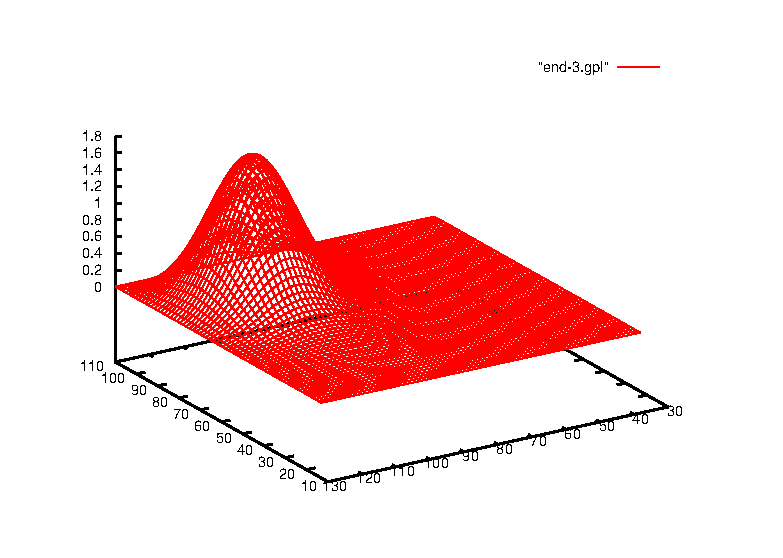
\includegraphics[width=15cm]{img/extension-barrier.eps}
}
\caption{Valore della soluzione di una \emph{call up\&out}, con barriere $H_1=110$, $H_2=130$.}
\label{fig:barrier}
\end{center}
\end{figure}
\end{description}


\chapter{Conclusioni}
Al termine di questo elaborato siamo in grado di trarre le seguenti conclusioni.\\
%Siamo dunque giunti al termine di questo elaborato, ed \`e ora di trarre delle conclusioni.\\

Il primo punto su cui vorremmo soffermarci \`e il confronto fra le trasformazioni \emph{price} e \emph{log-price}: come abbiamo potuto vedere nel Capitolo 6, analizzando i risultati, la trasformazione \emph{price} in 2d si \`e dimostrata sorprendentemente veloce nella risoluzione del problema, mentre nel caso monodimensionale occorre fare delle considerazioni pi\`u delicate. Nonostante infatti il calcolo dell'integrale con \emph{price} sia algoritmicamente pi\`u veloce rispetto alla trasformazione \emph{log-price}, quest'ultima, complici la facile parallelizzazione e la veloce convergenza dell'integrale garantita dai nodi di Hermite e di Laguerre, risulta pi\`u veloce su un computer di media potenza, cio\`e con a disposizione 4 \emph{cores}.\\

Un altro punto su cui vorremmo spendere qualche parola riguarda il \emph{solver} iterativo che abbiamo scritto per il \emph{pricing} di opzioni americane. Anche in questo caso abbiamo ottenuto dei risultati contrastanti: per quanto riguarda il caso \emph{Black\&Scholes} senza \emph{mesh refinement} infatti le prestazioni sono ottime, anche migliori del \emph{solver} \textsf{UMFPACK} di \textsf{deal.ii} come dimostra il confronto fra i risultati nelle tabelle \ref{test1-1} e \ref{test3-1}, mentre quando introduciamo il \emph{mesh refinement} le prestazioni peggiorano molto, tanto che nel \emph{log-price} il \emph{solver} fatica addirittura a convergere al risultato corretto. Riteniamo che questi comportamenti contrastanti siano legate al condizionamento del problema: il nostro \emph{solver} infatti \`e molto semplice e non fa alcun test sulla matrice di sistema, e questo si traduce in prestazioni ottime quando la matrice \`e ben condizionata e prestazioni non buone quando \`e mal condizionata. Il \emph{solver} di \textsf{deal.ii} invece riteniamo che esegua dei test sulla matrice, impiegando anche del tempo aggiuntivo per risolvere il sistema, e applichi in ogni occasione il metodo migliore\footnote{Nella descrizione di \textsf{UMFPACK} infatti \`e scritto che questo \emph{tool} \`e un set di \emph{routine} per risolvere sistemi lineari asimmetrici, quindi non \`e semplicemente un \emph{solver}.}. Probabilmente, applicando dei condizionatori adatti, le prestazioni del nostro \emph{solver} iterativo potrebbero beneficiarne.\\

Dedichiamo poi qualche riga al confronto fra metodi alle differenze finite e metodi agli elementi finiti. Come gi\`a accennato in precedenza, non possiamo non annoverare fra i vantaggi degli elementi finiti il fatto che la soluzione \`e calcolata sull'intero dominio, e non solo su un numero finito di punti come nel caso delle differenze finite. Ci\`o permette quindi di ottenere una soluzione pi\`u ``pregiata'', utile anche nel caso in cui occorra calcolare le derivate della soluzione. A tal proposito \`e noto che gli elementi finiti riescano meglio rispetto alle differenze finite a descrivere cambi relativamente bruschi di inclinazione. L'adattamento di griglia infatti pu\`o essere adottato per il calcolo della soluzione anche con condizioni finali continue ma non derivabili, ottenendo cos\`i un risultato pi\`u preciso non solo nel prezzo, ma anche nelle misure di sensitivit\`a del derivato. Le cosiddette Greche, infatti, cio\`e i valori delle derivate prima e seconda della soluzione, possono essere calcolate con pi\`u precisione rispetto al caso delle differenze finite. Ovviamente il lato negativo degli elementi finiti \`e la difficolt\`a sia nel ricavare la formulazione debole, sia nell'implementare correttamente i vari algoritmi da un punto di vista di programmazione. Infatti, mentre con le differenze finite anche un problema in 2d \`e facilmente implementabile, con gli elementi finiti \`e molto complicato risolvere problemi multi dimensionali senza l'ausilio di una libreria esterna che si occupi di gestire gli elementi. La piccola libreria da noi scritta, con l'ausilio di \textsf{deal.ii}, nasconde parte di queste problematiche e permette di sviluppare codici agli elementi finiti in modo molto rapido, anche nel caso bidimensionale.\\

Infine ci soffermiamo a sottolineare la velocit\`a dei nostri codici rispetto a una semplice implementazione in \textsf{Matlab}. Nel caso integro-differenziale monodimensionale infatti, i nostri prezzi vengono calcolati in un terzo del tempo. Nel caso 2d, invece, abbiamo potuto confrontare i tempi solo con un caso \emph{Black\&Scholes} alle differenze finite, e anche in questo caso il nostro codice \`e due volte pi\`u veloce. Per quanto riguarda il problema con l'ostacolo, ovvero l'opzione americana, il confronto non regge: dovendo infatti scrivere un \emph{solver} all'interno dello \emph{script}, \textsf{Matlab} impiega moltissimo tempo, tanto \`e vero che il prezzo di una semplice PDE di \emph{Black\&Scholes} viene calcolato in 18 minuti, contro i nostri 0.88 secondi.
\clearpage
\addcontentsline{toc}{chapter}{Bibliografia}
%stile della bibliografia
\bibliographystyle{plain}
%questo specifica il file da usare
\bibliography{Fonti}

\iffalse
\begin{thebibliography}{9}
\bibitem{} R Cont, P Tankov. \emph{Financial Modelling with Jump Processes}. Chapman \& Hall, 2004.
\bibitem{} R Seydel. \emph{Tools for Computational Finance}. Springer, 2009.
\bibitem{} Y Achdou, O Pironneau. \emph{Computational Methods for Option Pricing}. SIAM, 2005.
\bibitem{} J Tao, L Xin, Y Zhengzhou. \emph{Finite Element Algorithms for Pricing 2-D Basket Options}. 2009.
\bibitem{} Z Jinghui. \emph{Multi-Asset Option Pricing with L\'evy process}. 2009.
\bibitem{} A Quarteroni. \emph{Modellistica numerica per problemi differenziali}. Springer, 2008.
\bibitem{} A Quarteroni, R Sacco, F Saleri. \emph{Matematica Numerica}. Springer, 2008.
\bibitem{} L Feng, V Linetsky, J L Morales, J Nocedal. \emph{On the Solution of Complementarity Problems Arising in American Options Pricing}. 2010.
\bibitem{} E Gamma, R Helm, R Johnson, V Vlissides. \emph{Design Patterns}. 1997.

\end{thebibliography}
\fi
\end{document}
